% Options for packages loaded elsewhere
\PassOptionsToPackage{unicode}{hyperref}
\PassOptionsToPackage{hyphens}{url}
%
\documentclass[
]{article}
\usepackage{amsmath,amssymb}
\usepackage{lmodern}
\usepackage{iftex}
\ifPDFTeX
  \usepackage[T1]{fontenc}
  \usepackage[utf8]{inputenc}
  \usepackage{textcomp} % provide euro and other symbols
\else % if luatex or xetex
  \usepackage{unicode-math}
  \defaultfontfeatures{Scale=MatchLowercase}
  \defaultfontfeatures[\rmfamily]{Ligatures=TeX,Scale=1}
\fi
% Use upquote if available, for straight quotes in verbatim environments
\IfFileExists{upquote.sty}{\usepackage{upquote}}{}
\IfFileExists{microtype.sty}{% use microtype if available
  \usepackage[]{microtype}
  \UseMicrotypeSet[protrusion]{basicmath} % disable protrusion for tt fonts
}{}
\makeatletter
\@ifundefined{KOMAClassName}{% if non-KOMA class
  \IfFileExists{parskip.sty}{%
    \usepackage{parskip}
  }{% else
    \setlength{\parindent}{0pt}
    \setlength{\parskip}{6pt plus 2pt minus 1pt}}
}{% if KOMA class
  \KOMAoptions{parskip=half}}
\makeatother
\usepackage{xcolor}
\usepackage[margin=1in]{geometry}
\usepackage{color}
\usepackage{fancyvrb}
\newcommand{\VerbBar}{|}
\newcommand{\VERB}{\Verb[commandchars=\\\{\}]}
\DefineVerbatimEnvironment{Highlighting}{Verbatim}{commandchars=\\\{\}}
% Add ',fontsize=\small' for more characters per line
\usepackage{framed}
\definecolor{shadecolor}{RGB}{248,248,248}
\newenvironment{Shaded}{\begin{snugshade}}{\end{snugshade}}
\newcommand{\AlertTok}[1]{\textcolor[rgb]{0.94,0.16,0.16}{#1}}
\newcommand{\AnnotationTok}[1]{\textcolor[rgb]{0.56,0.35,0.01}{\textbf{\textit{#1}}}}
\newcommand{\AttributeTok}[1]{\textcolor[rgb]{0.77,0.63,0.00}{#1}}
\newcommand{\BaseNTok}[1]{\textcolor[rgb]{0.00,0.00,0.81}{#1}}
\newcommand{\BuiltInTok}[1]{#1}
\newcommand{\CharTok}[1]{\textcolor[rgb]{0.31,0.60,0.02}{#1}}
\newcommand{\CommentTok}[1]{\textcolor[rgb]{0.56,0.35,0.01}{\textit{#1}}}
\newcommand{\CommentVarTok}[1]{\textcolor[rgb]{0.56,0.35,0.01}{\textbf{\textit{#1}}}}
\newcommand{\ConstantTok}[1]{\textcolor[rgb]{0.00,0.00,0.00}{#1}}
\newcommand{\ControlFlowTok}[1]{\textcolor[rgb]{0.13,0.29,0.53}{\textbf{#1}}}
\newcommand{\DataTypeTok}[1]{\textcolor[rgb]{0.13,0.29,0.53}{#1}}
\newcommand{\DecValTok}[1]{\textcolor[rgb]{0.00,0.00,0.81}{#1}}
\newcommand{\DocumentationTok}[1]{\textcolor[rgb]{0.56,0.35,0.01}{\textbf{\textit{#1}}}}
\newcommand{\ErrorTok}[1]{\textcolor[rgb]{0.64,0.00,0.00}{\textbf{#1}}}
\newcommand{\ExtensionTok}[1]{#1}
\newcommand{\FloatTok}[1]{\textcolor[rgb]{0.00,0.00,0.81}{#1}}
\newcommand{\FunctionTok}[1]{\textcolor[rgb]{0.00,0.00,0.00}{#1}}
\newcommand{\ImportTok}[1]{#1}
\newcommand{\InformationTok}[1]{\textcolor[rgb]{0.56,0.35,0.01}{\textbf{\textit{#1}}}}
\newcommand{\KeywordTok}[1]{\textcolor[rgb]{0.13,0.29,0.53}{\textbf{#1}}}
\newcommand{\NormalTok}[1]{#1}
\newcommand{\OperatorTok}[1]{\textcolor[rgb]{0.81,0.36,0.00}{\textbf{#1}}}
\newcommand{\OtherTok}[1]{\textcolor[rgb]{0.56,0.35,0.01}{#1}}
\newcommand{\PreprocessorTok}[1]{\textcolor[rgb]{0.56,0.35,0.01}{\textit{#1}}}
\newcommand{\RegionMarkerTok}[1]{#1}
\newcommand{\SpecialCharTok}[1]{\textcolor[rgb]{0.00,0.00,0.00}{#1}}
\newcommand{\SpecialStringTok}[1]{\textcolor[rgb]{0.31,0.60,0.02}{#1}}
\newcommand{\StringTok}[1]{\textcolor[rgb]{0.31,0.60,0.02}{#1}}
\newcommand{\VariableTok}[1]{\textcolor[rgb]{0.00,0.00,0.00}{#1}}
\newcommand{\VerbatimStringTok}[1]{\textcolor[rgb]{0.31,0.60,0.02}{#1}}
\newcommand{\WarningTok}[1]{\textcolor[rgb]{0.56,0.35,0.01}{\textbf{\textit{#1}}}}
\usepackage{graphicx}
\makeatletter
\def\maxwidth{\ifdim\Gin@nat@width>\linewidth\linewidth\else\Gin@nat@width\fi}
\def\maxheight{\ifdim\Gin@nat@height>\textheight\textheight\else\Gin@nat@height\fi}
\makeatother
% Scale images if necessary, so that they will not overflow the page
% margins by default, and it is still possible to overwrite the defaults
% using explicit options in \includegraphics[width, height, ...]{}
\setkeys{Gin}{width=\maxwidth,height=\maxheight,keepaspectratio}
% Set default figure placement to htbp
\makeatletter
\def\fps@figure{htbp}
\makeatother
\setlength{\emergencystretch}{3em} % prevent overfull lines
\providecommand{\tightlist}{%
  \setlength{\itemsep}{0pt}\setlength{\parskip}{0pt}}
\setcounter{secnumdepth}{-\maxdimen} % remove section numbering
\usepackage{booktabs}
\usepackage{longtable}
\usepackage{array}
\usepackage{multirow}
\usepackage{wrapfig}
\usepackage{float}
\usepackage{colortbl}
\usepackage{pdflscape}
\usepackage{tabu}
\usepackage{threeparttable}
\usepackage{threeparttablex}
\usepackage[normalem]{ulem}
\usepackage{makecell}
\usepackage{xcolor}
\usepackage{siunitx}

  \newcolumntype{d}{S[
    input-open-uncertainty=,
    input-close-uncertainty=,
    parse-numbers = false,
    table-align-text-pre=false,
    table-align-text-post=false
  ]}
  
\ifLuaTeX
  \usepackage{selnolig}  % disable illegal ligatures
\fi
\IfFileExists{bookmark.sty}{\usepackage{bookmark}}{\usepackage{hyperref}}
\IfFileExists{xurl.sty}{\usepackage{xurl}}{} % add URL line breaks if available
\urlstyle{same} % disable monospaced font for URLs
\hypersetup{
  pdftitle={Problem Set 2: Regression},
  pdfauthor={Jamie Esmond},
  hidelinks,
  pdfcreator={LaTeX via pandoc}}

\title{Problem Set 2: Regression}
\author{Jamie Esmond}
\date{01/27/2023}

\begin{document}
\maketitle

{
\setcounter{tocdepth}{2}
\tableofcontents
}
\begin{Shaded}
\begin{Highlighting}[]
\FunctionTok{library}\NormalTok{(tidyverse)}
\FunctionTok{library}\NormalTok{(broom)}
\FunctionTok{library}\NormalTok{(modelsummary)}
\FunctionTok{library}\NormalTok{(kableExtra)}

\CommentTok{\# Load penguins data}
\NormalTok{penguins }\OtherTok{\textless{}{-}} \FunctionTok{read\_csv}\NormalTok{(}\StringTok{"data/penguins.csv"}\NormalTok{)}
\end{Highlighting}
\end{Shaded}

\hypertarget{task-1-penguins}{%
\section{Task 1: Penguins}\label{task-1-penguins}}

Between 2007 and 2009, researchers collected data on penguins in three
islands in the Palmer Archipelago in Antarctica: Biscoe, Dream, and
Torgersen. The \texttt{penguins} dataset has data for 342 penguins from
3 different species: Chinstrap, Gentoo, and Adélie. It includes the
following variables:

\begin{itemize}
\tightlist
\item
  \texttt{species}: The penguin's species (Chinstrap, Gentoo, and
  Adélie)
\item
  \texttt{island}: The island where the penguin lives (Biscoe, Dream,
  and Torgersen)
\item
  \texttt{bill\_length\_mm}: The length of the penguin's bill, in
  millimeters (distance from the penguin's face to the tip of the bill)
\item
  \texttt{bill\_depth\_mm}: The depth of the penguin's bill, in
  millimeters (height of the bill; distance from the bottom of the bill
  to the top of the bill)
\item
  \texttt{flipper\_length\_mm}: The length of the penguin's flippers, in
  millimeters
\item
  \texttt{body\_mass\_g}: The weight of the penguin, in grams
\item
  \texttt{sex}: The sex of the penguin
\item
  \texttt{year}: The year the observation was made
\end{itemize}

\hypertarget{exploratory-analysis}{%
\subsection{Exploratory analysis}\label{exploratory-analysis}}

What is the relationship between penguin weight and bill depth? This
plot shows some initial trends:

\begin{Shaded}
\begin{Highlighting}[]
\FunctionTok{ggplot}\NormalTok{(}\AttributeTok{data =}\NormalTok{ penguins, }
       \FunctionTok{aes}\NormalTok{(}\AttributeTok{x =}\NormalTok{ bill\_depth\_mm, }\AttributeTok{y =}\NormalTok{ body\_mass\_g)) }\SpecialCharTok{+}
  \FunctionTok{geom\_point}\NormalTok{() }\SpecialCharTok{+}
  \FunctionTok{labs}\NormalTok{(}\AttributeTok{x =} \StringTok{"Bill Depth (mm)"}\NormalTok{, }
       \AttributeTok{y =} \StringTok{"Body Mass (g)"}\NormalTok{)}
\end{Highlighting}
\end{Shaded}

\begin{center}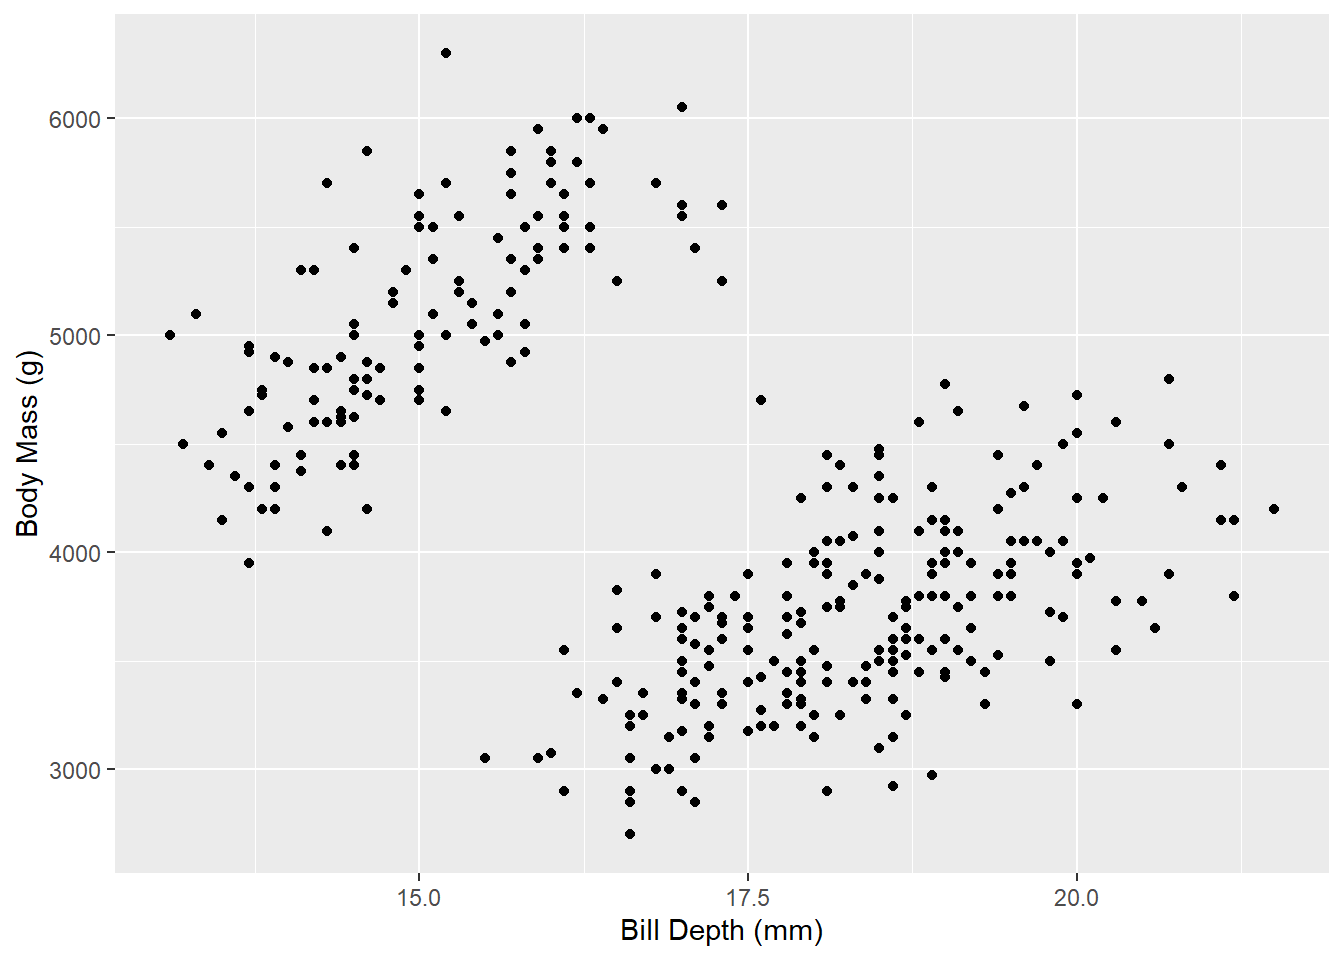
\includegraphics{Jamie-Esmond_Problem-Set-2_files/figure-latex/plot-penguin-weight-depth-1} \end{center}

\textbf{This plot shows that, generally, as bill depth grows, body mass
increases assuming whatever is causing the two separate clusters to
appear, which is unclear from this plot, is controlled for. These
clusters indicate that there may be other factors influencing the body
mass of penguins.}

Make a new plot that colors these points by species. What can you tell
about the relationship between bill depth and penguin weight?

\begin{Shaded}
\begin{Highlighting}[]
\FunctionTok{ggplot}\NormalTok{(}\AttributeTok{data =}\NormalTok{ penguins, }
       \FunctionTok{aes}\NormalTok{(}\AttributeTok{x =}\NormalTok{ bill\_depth\_mm, }\AttributeTok{y =}\NormalTok{ body\_mass\_g)) }\SpecialCharTok{+}
  \FunctionTok{geom\_point}\NormalTok{(}\AttributeTok{mapping =} \FunctionTok{aes}\NormalTok{(}\AttributeTok{color =}\NormalTok{ species)) }\SpecialCharTok{+}
  \FunctionTok{labs}\NormalTok{(}\AttributeTok{x =} \StringTok{"Bill Depth (mm)"}\NormalTok{, }
       \AttributeTok{y =} \StringTok{"Body Mass (g)"}\NormalTok{)}
\end{Highlighting}
\end{Shaded}

\begin{center}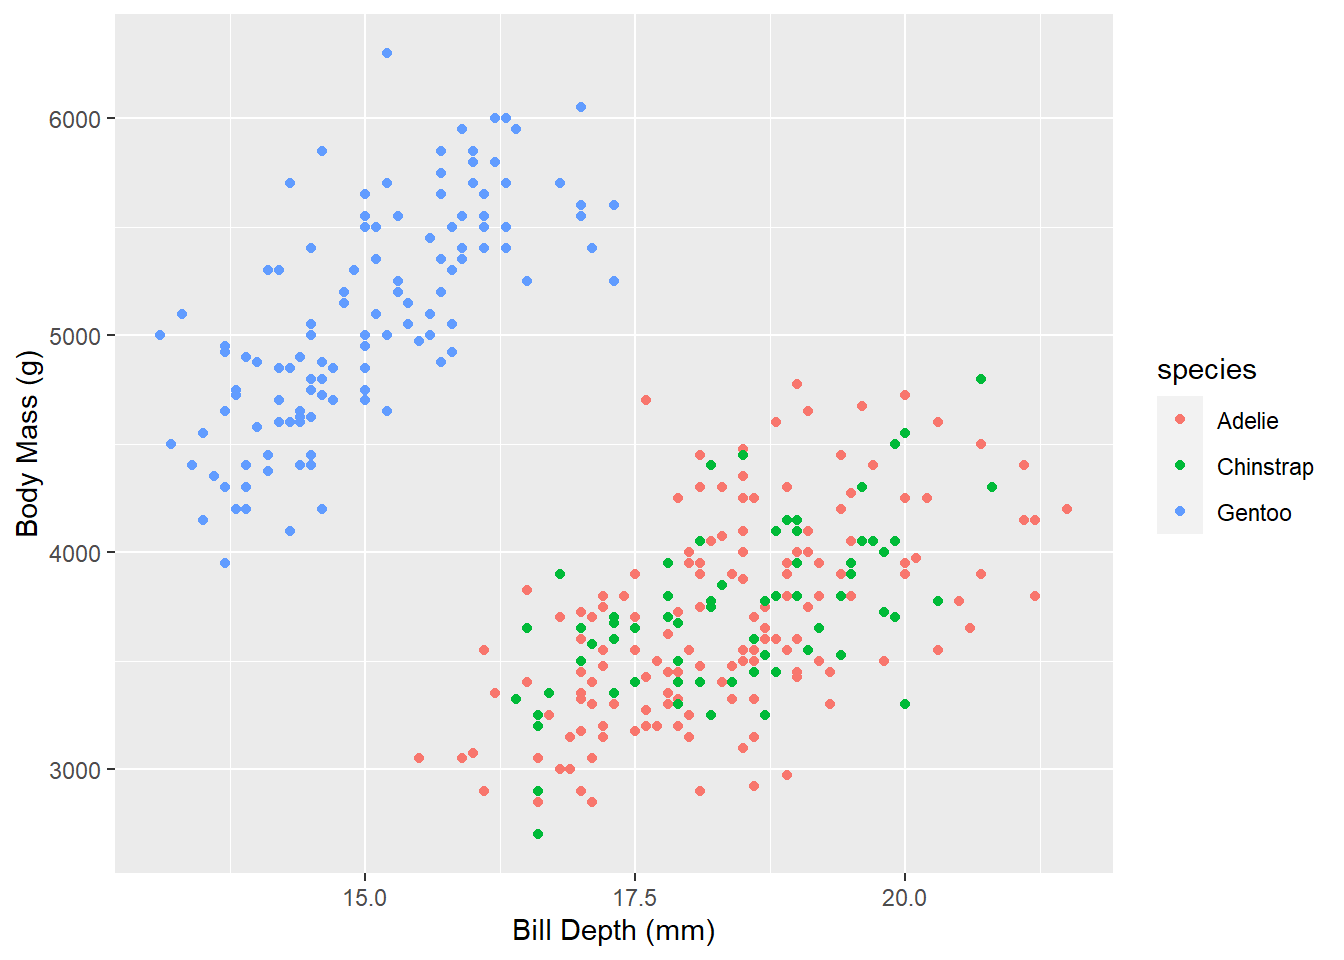
\includegraphics{Jamie-Esmond_Problem-Set-2_files/figure-latex/plot-penguin-weight-depth-by-species-1} \end{center}

\textbf{This plot clearly shows that Gentoo penguins have smaller bill
depth than Adelie and Chinstrap penguins, but within there own species,
bill depth still has a positive correlation to body mass. Though the
Adelie and Chinstrap penguins are generally smaller in body mass and
bill depth than Gentoo penguins, within their species, there is still a
postive correlation between bill depth and body mass.}

Add a \texttt{geom\_smooth()} layer to the plot and make sure it uses a
straight line (hint: include \texttt{method="lm"} in the function). What
does this tell you about the relationship between bill depth and body
mass?

\begin{Shaded}
\begin{Highlighting}[]
\FunctionTok{ggplot}\NormalTok{(}\AttributeTok{data =}\NormalTok{ penguins, }
       \FunctionTok{aes}\NormalTok{(}\AttributeTok{x =}\NormalTok{ bill\_depth\_mm, }\AttributeTok{y =}\NormalTok{ body\_mass\_g, }\AttributeTok{color =}\NormalTok{ species)) }\SpecialCharTok{+}
  \FunctionTok{geom\_point}\NormalTok{() }\SpecialCharTok{+}
  \FunctionTok{geom\_smooth}\NormalTok{(}\AttributeTok{method =} \StringTok{"lm"}\NormalTok{) }\SpecialCharTok{+}
  \FunctionTok{labs}\NormalTok{(}\AttributeTok{x =} \StringTok{"Bill Depth (mm)"}\NormalTok{, }
       \AttributeTok{y =} \StringTok{"Body Mass (g)"}\NormalTok{)}
\end{Highlighting}
\end{Shaded}

\begin{verbatim}
## `geom_smooth()` using formula = 'y ~ x'
\end{verbatim}

\begin{center}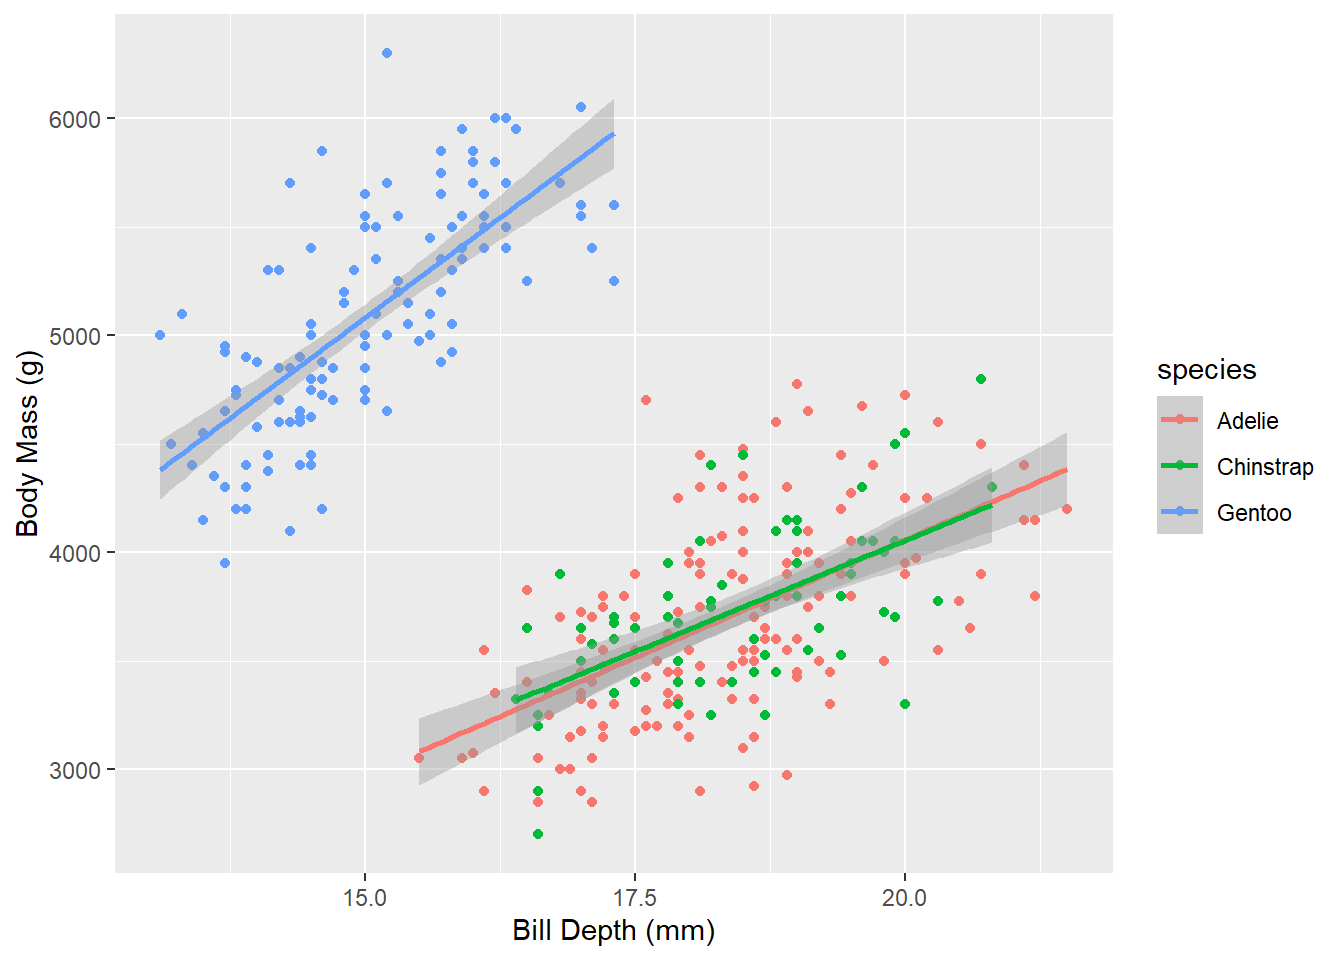
\includegraphics{Jamie-Esmond_Problem-Set-2_files/figure-latex/plot-penguin-weight-depth-by-species-with-lines-1} \end{center}

\textbf{As stated earlier, this plot shows even more clearly the upward
slope of the trendline, indicating a positive relationship between bill
depth and body mass.}

Change the plot so that there's a single line for all the points instead
of one line per species. How does the slope of this single line differ
from the slopes of the species specific lines? \textbf{\emph{Why??}}

\begin{Shaded}
\begin{Highlighting}[]
\FunctionTok{ggplot}\NormalTok{(}\AttributeTok{data =}\NormalTok{ penguins, }
       \FunctionTok{aes}\NormalTok{(}\AttributeTok{x =}\NormalTok{ bill\_depth\_mm, }\AttributeTok{y =}\NormalTok{ body\_mass\_g)) }\SpecialCharTok{+}
  \FunctionTok{geom\_point}\NormalTok{() }\SpecialCharTok{+}
  \FunctionTok{geom\_smooth}\NormalTok{(}\AttributeTok{method =} \StringTok{"lm"}\NormalTok{) }\SpecialCharTok{+}
  \FunctionTok{labs}\NormalTok{(}\AttributeTok{x =} \StringTok{"Bill Depth (mm)"}\NormalTok{, }
       \AttributeTok{y =} \StringTok{"Body Mass (g)"}\NormalTok{)}
\end{Highlighting}
\end{Shaded}

\begin{verbatim}
## `geom_smooth()` using formula = 'y ~ x'
\end{verbatim}

\begin{center}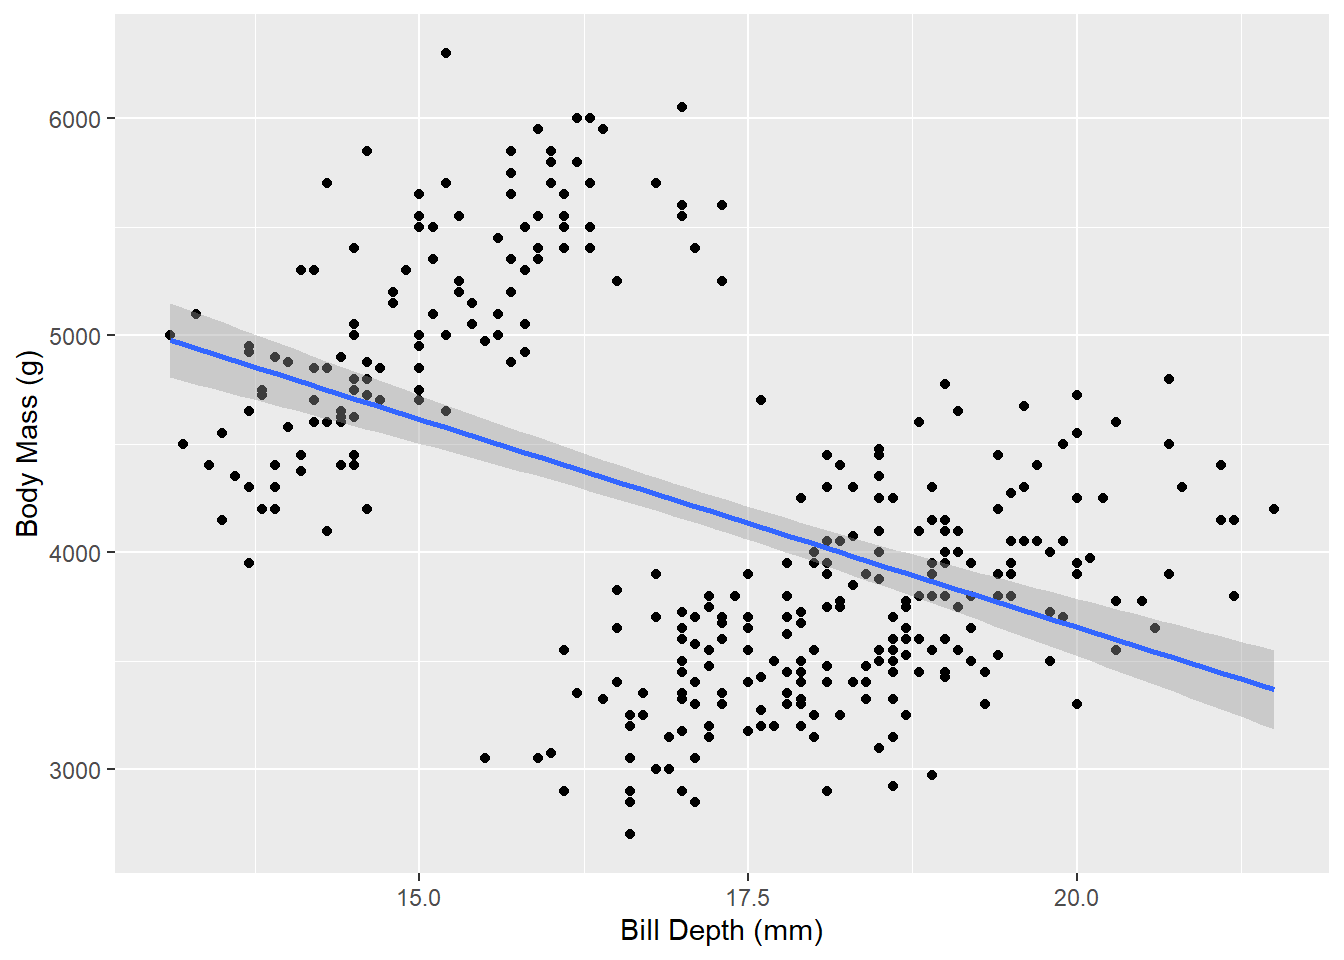
\includegraphics{Jamie-Esmond_Problem-Set-2_files/figure-latex/plot-penguin-weight-depth-by-species-with-one-line-1} \end{center}

\textbf{When species is not controlled for, the there is an overall
downward slope, indicating a negative relationship between bill depth
and body mass. This is because there are more penguins in the sample
from either Adelie or Chinstrap species than from the Gentoo species.
Since the bill depth is higher for the first two species, but those
species also generally have a smaller body mass, it weights the
distribution in a misleading way. }

What is the relationship between flipper length and body mass? Make
another plot with \texttt{flipper\_length\_mm} on the x-axis,
\texttt{body\_mass\_g} on the y-axis, and points colored by
\texttt{species}.

\begin{Shaded}
\begin{Highlighting}[]
\FunctionTok{ggplot}\NormalTok{(}\AttributeTok{data =}\NormalTok{ penguins, }
       \FunctionTok{aes}\NormalTok{(}\AttributeTok{x =}\NormalTok{ flipper\_length\_mm, }\AttributeTok{y =}\NormalTok{ body\_mass\_g, }\AttributeTok{color =}\NormalTok{ species)) }\SpecialCharTok{+}
  \FunctionTok{geom\_point}\NormalTok{() }\SpecialCharTok{+}
  \FunctionTok{geom\_smooth}\NormalTok{(}\AttributeTok{method =} \StringTok{"lm"}\NormalTok{) }\SpecialCharTok{+}
  \FunctionTok{labs}\NormalTok{(}\AttributeTok{x =} \StringTok{"Flipper Length (mm)"}\NormalTok{, }
       \AttributeTok{y =} \StringTok{"Body Mass (g)"}\NormalTok{)}
\end{Highlighting}
\end{Shaded}

\begin{verbatim}
## `geom_smooth()` using formula = 'y ~ x'
\end{verbatim}

\begin{center}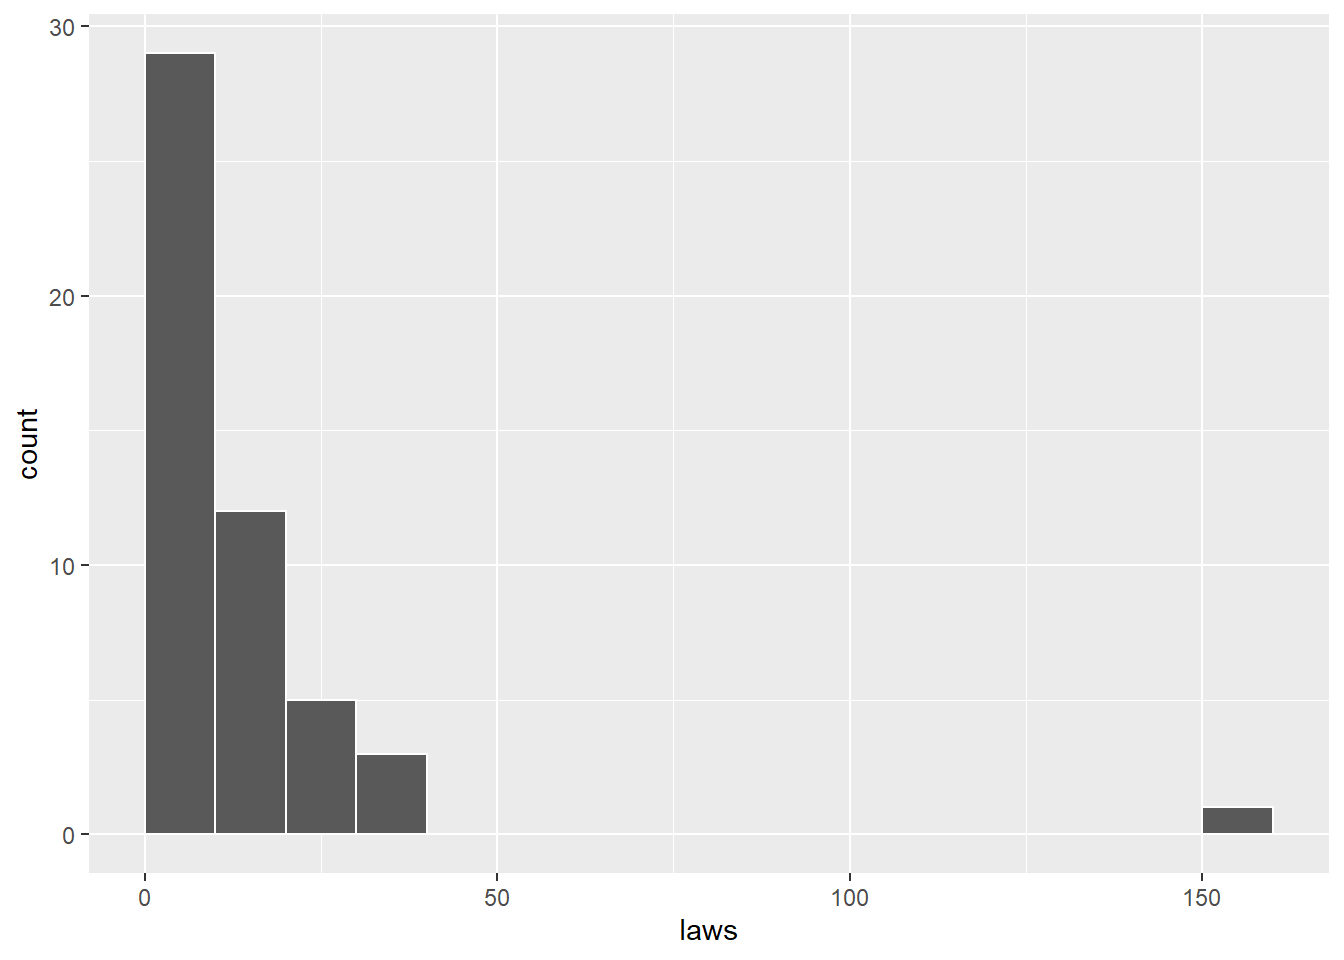
\includegraphics{Jamie-Esmond_Problem-Set-2_files/figure-latex/unnamed-chunk-1-1} \end{center}

\textbf{This plot shows that there is a positive relationship between
flipper length and body mass. }

Facet the plot by island (\texttt{island})

\begin{Shaded}
\begin{Highlighting}[]
\FunctionTok{ggplot}\NormalTok{(}\AttributeTok{data =}\NormalTok{ penguins,}
       \FunctionTok{aes}\NormalTok{(}\AttributeTok{x =}\NormalTok{ flipper\_length\_mm, }\AttributeTok{y =}\NormalTok{ body\_mass\_g, }\AttributeTok{color =}\NormalTok{ species)) }\SpecialCharTok{+}
  \FunctionTok{geom\_point}\NormalTok{() }\SpecialCharTok{+}
  \FunctionTok{facet\_wrap}\NormalTok{(}\FunctionTok{vars}\NormalTok{(island)) }\SpecialCharTok{+}
  \FunctionTok{labs}\NormalTok{(}\AttributeTok{x =} \StringTok{"Flipper Length (mm)"}\NormalTok{, }
       \AttributeTok{y =} \StringTok{"Body Mass (g)"}\NormalTok{)}
\end{Highlighting}
\end{Shaded}

\begin{center}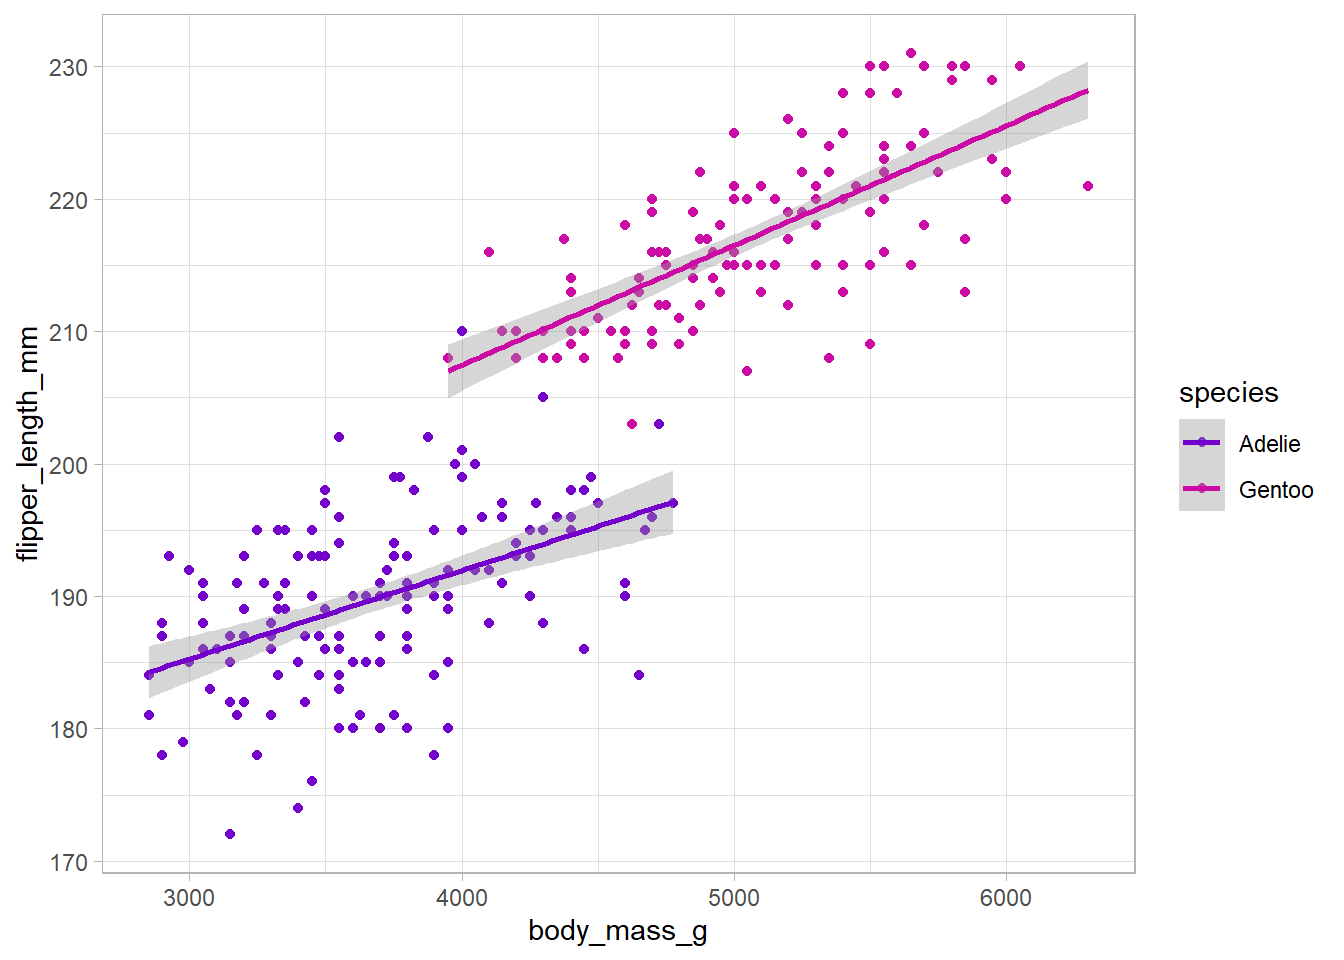
\includegraphics{Jamie-Esmond_Problem-Set-2_files/figure-latex/unnamed-chunk-2-1} \end{center}

Tell a story about the relationship between flipper length and weight in
these three penguin species.

\textbf{As flipper length increases, body mass also increases. Though
the Gentoo penguins seem to be larger in general, both in flipper length
and body mass, the trend is consistent among all species that with
longer flippers there is a higher body mass.}

Tell a story about the distribution of penguins across the three
islands.

\textbf{Adelie penguins are found on all three islands, but Gentoo
penguins and Chinstrap penguins are only found on Biscoe and Dream,
respectively. Biscoe island contains both Adelie and Gentoo penguins.
Dream island contains both Adelie and Chinstrap penguins. Torgersen
island contains only Adelie penguins. If the species were not coded by
color in these plots, one might conclude that penguins are larger on the
island of Biscoe because the overall average body mass of penguins on
that island is larger. The colors help convey that the difference in
size is probably better explained by the species of penguin than the
location.}

\hypertarget{models}{%
\subsection{Models}\label{models}}

\hypertarget{predicting-weight-with-bill-depth}{%
\subsubsection{Predicting weight with bill
depth}\label{predicting-weight-with-bill-depth}}

Does bill depth predict penguin weight?

\begin{Shaded}
\begin{Highlighting}[]
\NormalTok{model\_depth\_weight }\OtherTok{\textless{}{-}} \FunctionTok{lm}\NormalTok{(body\_mass\_g }\SpecialCharTok{\textasciitilde{}}\NormalTok{ bill\_depth\_mm,}
                         \AttributeTok{data =}\NormalTok{ penguins)}

\FunctionTok{tidy}\NormalTok{(model\_depth\_weight, }\AttributeTok{conf.int =} \ConstantTok{TRUE}\NormalTok{)}
\end{Highlighting}
\end{Shaded}

\begin{verbatim}
## # A tibble: 2 x 7
##   term          estimate std.error statistic  p.value conf.low conf.high
##   <chr>            <dbl>     <dbl>     <dbl>    <dbl>    <dbl>     <dbl>
## 1 (Intercept)      7489.     335.      22.3  1.13e-68    6829.     8148.
## 2 bill_depth_mm    -192.      19.4     -9.87 2.28e-20    -230.     -153.
\end{verbatim}

\begin{Shaded}
\begin{Highlighting}[]
\FunctionTok{glance}\NormalTok{(model\_depth\_weight)}
\end{Highlighting}
\end{Shaded}

\begin{verbatim}
## # A tibble: 1 x 12
##   r.squared adj.r.squa~1 sigma stati~2  p.value    df logLik   AIC   BIC devia~3
##       <dbl>        <dbl> <dbl>   <dbl>    <dbl> <dbl>  <dbl> <dbl> <dbl>   <dbl>
## 1     0.223        0.220  708.    97.4 2.28e-20     1 -2729. 5463. 5475.  1.70e8
## # ... with 2 more variables: df.residual <int>, nobs <int>, and abbreviated
## #   variable names 1: adj.r.squared, 2: statistic, 3: deviance
\end{verbatim}

What happens as bills get taller? Is the association statistically
significant? How confident are you about these results? (Hint: look at
the \(R^2\))

\textbf{The intercept is 7488.65, which means that the average penguin
will have a body mass of 7488.65 grams when the bill depth is 0 mm. This
does not mean much since no penguin has a bill depth of 0 mm. The slope
of bill\_depth\_mm is -191.64, which means that a 1 mm increase in bill
depth is associated with a 191.64 gram decrease in body mass, on
average, without controlling for any other factors. The association is
statistically significant because the p value is virtually zero. The
\(R^2\) here is 0.223, which means that bill depth explains only 22.3\%
of the variation in penguin body mass. }

\hypertarget{predicting-weight-with-bill-depth-and-flipper-length}{%
\subsubsection{Predicting weight with bill depth and flipper
length}\label{predicting-weight-with-bill-depth-and-flipper-length}}

RUN A MODEL that predicts weight with bill depth and flipper length
(i.e.~body\_mass\_g \textasciitilde{} bill\_depth\_mm +
flipper\_length\_mm)

\begin{Shaded}
\begin{Highlighting}[]
\NormalTok{model\_weight\_depth\_flipper }\OtherTok{\textless{}{-}} \FunctionTok{lm}\NormalTok{(body\_mass\_g }\SpecialCharTok{\textasciitilde{}} 
\NormalTok{                                   bill\_depth\_mm }\SpecialCharTok{+} 
\NormalTok{                                   flipper\_length\_mm,}
                         \AttributeTok{data =}\NormalTok{ penguins)}

\FunctionTok{tidy}\NormalTok{(model\_weight\_depth\_flipper, }\AttributeTok{conf.int =} \ConstantTok{TRUE}\NormalTok{)}
\end{Highlighting}
\end{Shaded}

\begin{verbatim}
## # A tibble: 3 x 7
##   term              estimate std.error statistic  p.value conf.low conf.high
##   <chr>                <dbl>     <dbl>     <dbl>    <dbl>    <dbl>     <dbl>
## 1 (Intercept)        -6542.     541.      -12.1  2.99e-28 -7606.     -5478. 
## 2 bill_depth_mm         22.6     13.3       1.70 8.92e- 2    -3.49      48.8
## 3 flipper_length_mm     51.5      1.87     27.6  7.72e-89    47.9       55.2
\end{verbatim}

\begin{Shaded}
\begin{Highlighting}[]
\FunctionTok{glance}\NormalTok{(model\_weight\_depth\_flipper)}
\end{Highlighting}
\end{Shaded}

\begin{verbatim}
## # A tibble: 1 x 12
##   r.squared adj.r.squ~1 sigma stati~2   p.value    df logLik   AIC   BIC devia~3
##       <dbl>       <dbl> <dbl>   <dbl>     <dbl> <dbl>  <dbl> <dbl> <dbl>   <dbl>
## 1     0.761       0.760  393.    540. 4.23e-106     2 -2527. 5062. 5077.  5.24e7
## # ... with 2 more variables: df.residual <int>, nobs <int>, and abbreviated
## #   variable names 1: adj.r.squared, 2: statistic, 3: deviance
\end{verbatim}

Did the size of the bill depth coefficient change after controlling for
flipper length?

\textbf{The intercept is -6541.91, which means that the average penguin
will have a body mass of -6541.91 grams when the bill depth and the
flipper length is 0 mm. This does not mean much since a penguin cannot
have a negative weight, and no penguin has a bill depth or flipper
length of 0 mm. The slope of bill\_depth\_mm is now 22.63, which means
that a 1 mm increase in bill depth is associated with a 22.63 gram
increase in body mass, on average, when flipper length is held constant.
The slope of flipper\_length\_mm is 51.54, which means that a 1 mm
increase in flipper length is associated with a 51.54 gram increase in
body mass, on average, when bill depth is held constant. The coefficient
for bill\_depth\_mm completely changed directions, now indicating a
positive association between the two variables. The association is still
statistically significant because the p value is still virtually zero,
even though the correlation is now in a different direction. The
adjusted \(R^2\) here is 0.76, which means that bill depth and flipper
length explain 76\% of the variation in penguin body mass.}

\hypertarget{predicting-weight-with-bill-depth-flipper-length-and-species}{%
\subsubsection{Predicting weight with bill depth, flipper length, and
species}\label{predicting-weight-with-bill-depth-flipper-length-and-species}}

RUN A MODEL that predicts weight with bill depth, flipper length, and
species.

\begin{Shaded}
\begin{Highlighting}[]
\NormalTok{model\_weight\_depth\_flipper\_species }\OtherTok{\textless{}{-}} \FunctionTok{lm}\NormalTok{(body\_mass\_g }\SpecialCharTok{\textasciitilde{}} 
\NormalTok{                                          bill\_depth\_mm }\SpecialCharTok{+} 
\NormalTok{                                          flipper\_length\_mm }\SpecialCharTok{+} 
\NormalTok{                                          species,}
                                          \AttributeTok{data =}\NormalTok{ penguins)}

\FunctionTok{tidy}\NormalTok{(model\_weight\_depth\_flipper\_species, }\AttributeTok{conf.int =} \ConstantTok{TRUE}\NormalTok{)}
\end{Highlighting}
\end{Shaded}

\begin{verbatim}
## # A tibble: 5 x 7
##   term              estimate std.error statistic  p.value conf.low conf.high
##   <chr>                <dbl>     <dbl>     <dbl>    <dbl>    <dbl>     <dbl>
## 1 (Intercept)        -4527.     517.       -8.76 9.87e-17  -5544.    -3510. 
## 2 bill_depth_mm        182.      18.4       9.93 1.45e-20    146.      218. 
## 3 flipper_length_mm     25.7      3.10      8.30 2.63e-15     19.6      31.8
## 4 speciesChinstrap    -132.      51.4      -2.57 1.07e- 2   -233.      -30.9
## 5 speciesGentoo       1289.     133.        9.71 8.28e-20   1028.     1550.
\end{verbatim}

\begin{Shaded}
\begin{Highlighting}[]
\FunctionTok{glance}\NormalTok{(model\_weight\_depth\_flipper\_species)}
\end{Highlighting}
\end{Shaded}

\begin{verbatim}
## # A tibble: 1 x 12
##   r.squared adj.r.squ~1 sigma stati~2   p.value    df logLik   AIC   BIC devia~3
##       <dbl>       <dbl> <dbl>   <dbl>     <dbl> <dbl>  <dbl> <dbl> <dbl>   <dbl>
## 1     0.832       0.830  331.    417. 4.66e-129     4 -2467. 4946. 4969.  3.69e7
## # ... with 2 more variables: df.residual <int>, nobs <int>, and abbreviated
## #   variable names 1: adj.r.squared, 2: statistic, 3: deviance
\end{verbatim}

What do the species coefficients mean? Did the bill depth coefficient
change after controlling for both flipper length and species?

\textbf{The intercept is -4526.89, which means that the average penguin
will have a body mass of -4526.89 grams when the bill depth and the
flipper length is 0 mm and the species is Adelie (the reference group).
This does not mean much since a penguin cannot have a negative weight,
and no penguin has a bill depth or flipper length of 0 mm. The slope of
bill\_depth\_mm is now 182.36, which means that a 1 mm increase in bill
depth is associated with a 182.36 gram increase in body mass, on
average, when flipper length and species are held constant. The slope of
flipper\_length\_mm is now 25.7, which means that a 1 mm increase in
flipper length is associated with a 25.7 gram increase in body mass, on
average, when bill depth and species are held constant. The coefficient
for bill\_depth\_mm became even higher, indicating an even stronger
positive association between the two variables, hold the other constant.
The coefficient for Chinstrap is -131.97, which means that controlling
for bill depth and flipper length, Chinstrap penguins are 131.97 grams
lighter than Adelie penguins. The coefficient for Gentoo is 1288.97,
which means that controlling for bill depth and flipper length, Gentoo
penguins are 1288.97 grams heavier than Adelie penguins. The association
for all variables is statistically significant because the p values are
all virtually zero. The adjusted \(R^2\) here is 0.83, which means that
bill depth, flipper length, and species explain 83\% of the variation in
penguin body mass.}

\hypertarget{all-models-at-the-same-time}{%
\subsection{All models at the same
time}\label{all-models-at-the-same-time}}

\begin{Shaded}
\begin{Highlighting}[]
\CommentTok{\# Right now there\textquotesingle{}s only one model here. Add the others from above (whatever you}
\CommentTok{\# called them) like so: }
\CommentTok{\# modelsummary(list(model\_depth\_weight, some\_other\_model, yet\_another\_model, etc))}


\NormalTok{notes }\OtherTok{\textless{}{-}} \FunctionTok{c}\NormalTok{(}\StringTok{"t statistics in parentheses}\SpecialCharTok{\textbackslash{}n}\StringTok{"}\NormalTok{,}
           \StringTok{"+ p \textless{} 0.1, * p \textless{} 0.05, ** p \textless{} 0.01, *** p \textless{} 0.001"}\NormalTok{)}

\FunctionTok{modelsummary}\NormalTok{(}\FunctionTok{list}\NormalTok{(}\StringTok{"Model 1"}\OtherTok{=}\NormalTok{model\_depth\_weight, }
                  \StringTok{"Model 2"}\OtherTok{=}\NormalTok{model\_weight\_depth\_flipper, }
                  \StringTok{"Model 3"}\OtherTok{=}\NormalTok{model\_weight\_depth\_flipper\_species),}
             \AttributeTok{coef\_rename =} \FunctionTok{c}\NormalTok{(}\AttributeTok{bill\_depth\_mm =} \StringTok{"Bill Depth (mm)"}\NormalTok{, }
                             \AttributeTok{flipper\_length\_mm =} \StringTok{"Flipper Length (mm)"}\NormalTok{, }
                             \AttributeTok{speciesChinstrap =} \StringTok{"Chinstrap"}\NormalTok{, }
                             \AttributeTok{speciesGentoo =} \StringTok{"Gentoo"}\NormalTok{),}
             \AttributeTok{output =} \StringTok{"kableExtra"}\NormalTok{,}
             \AttributeTok{estimate =} \StringTok{"\{estimate\} \{stars\}"}\NormalTok{,}
             \AttributeTok{statistic =} \StringTok{"statistic"}\NormalTok{,}
             \AttributeTok{title =} \StringTok{"Penguin Models"}\NormalTok{,}
             \AttributeTok{fmt =}  \DecValTok{2}\NormalTok{) }\SpecialCharTok{\%\textgreater{}\%} 
  \FunctionTok{row\_spec}\NormalTok{(}\FunctionTok{c}\NormalTok{(}\DecValTok{1}\NormalTok{,}\DecValTok{3}\NormalTok{,}\DecValTok{5}\NormalTok{,}\DecValTok{7}\NormalTok{,}\DecValTok{9}\NormalTok{), }\AttributeTok{background =} \StringTok{"lightblue"}\NormalTok{) }\SpecialCharTok{\%\textgreater{}\%} 
  \FunctionTok{footnote}\NormalTok{(}\AttributeTok{general =}\NormalTok{ notes, }\AttributeTok{footnote\_as\_chunk =} \ConstantTok{TRUE}\NormalTok{)}
\end{Highlighting}
\end{Shaded}

\begin{table}

\caption{\label{tab:all-penguin-models}Penguin Models}
\centering
\begin{tabular}[t]{lccc}
\toprule
  & Model 1 & Model 2 & Model 3\\
\midrule
\cellcolor{lightblue}{(Intercept)} & \cellcolor{lightblue}{\num{7488.65} ***} & \cellcolor{lightblue}{\num{-6541.91} ***} & \cellcolor{lightblue}{\num{-4526.89} ***}\\
 & (\num{22.34}) & (\num{-12.10}) & (\num{-8.76})\\
\cellcolor{lightblue}{Bill Depth (mm)} & \cellcolor{lightblue}{\num{-191.64} ***} & \cellcolor{lightblue}{\num{22.63} +} & \cellcolor{lightblue}{\num{182.36} ***}\\
 & (\num{-9.87}) & (\num{1.70}) & (\num{9.93})\\
\cellcolor{lightblue}{Flipper Length (mm)} & \cellcolor{lightblue}{} & \cellcolor{lightblue}{\num{51.54} ***} & \cellcolor{lightblue}{\num{25.70} ***}\\
 &  & (\num{27.64}) & (\num{8.30})\\
\cellcolor{lightblue}{Chinstrap} & \cellcolor{lightblue}{} & \cellcolor{lightblue}{} & \cellcolor{lightblue}{\num{-131.97} *}\\
 &  &  & (\num{-2.57})\\
\cellcolor{lightblue}{Gentoo} & \cellcolor{lightblue}{} & \cellcolor{lightblue}{} & \cellcolor{lightblue}{\num{1288.97} ***}\\
 &  &  & (\num{9.71})\\
\midrule
Num.Obs. & \num{342} & \num{342} & \num{342}\\
R2 & \num{0.223} & \num{0.761} & \num{0.832}\\
R2 Adj. & \num{0.220} & \num{0.760} & \num{0.830}\\
AIC & \num{5463.3} & \num{5061.9} & \num{4945.7}\\
BIC & \num{5474.8} & \num{5077.3} & \num{4968.7}\\
Log.Lik. & \num{-2728.667} & \num{-2526.968} & \num{-2466.846}\\
RMSE & \num{706.00} & \num{391.45} & \num{328.34}\\
\bottomrule
\multicolumn{4}{l}{\rule{0pt}{1em}\textit{Note: } makecell[l]{t statistics in parentheses\} + p < 0.1, * p < 0.05, ** p < 0.01, *** p < 0.001}\\
\end{tabular}
\end{table}

\begin{center}\rule{0.5\linewidth}{0.5pt}\end{center}

\hypertarget{task-2-food-access-and-mortality}{%
\section{Task 2: Food access and
mortality}\label{task-2-food-access-and-mortality}}

\begin{Shaded}
\begin{Highlighting}[]
\CommentTok{\# Make sure you look at this dataset by clicking on its name in the Environment}
\CommentTok{\# panel in RStudio. Sort some of the different columns and look around to get a}
\CommentTok{\# feel for what\textquotesingle{}s in the data}
\NormalTok{food\_health }\OtherTok{\textless{}{-}} \FunctionTok{read\_csv}\NormalTok{(}\StringTok{"data/food\_health\_politics.csv"}\NormalTok{) }
\end{Highlighting}
\end{Shaded}

\begin{verbatim}
## Rows: 3143 Columns: 26
## -- Column specification --------------------------------------------------------
## Delimiter: ","
## chr  (2): state, county
## dbl (24): FIPS, low_access_pop, low_access_change, pct_low_access_pop, child...
## 
## i Use `spec()` to retrieve the full column specification for this data.
## i Specify the column types or set `show_col_types = FALSE` to quiet this message.
\end{verbatim}

We're interested in looking at the relationships between food access,
mortality, and politics. Do do this, we look at data from three
different sources:

\begin{itemize}
\tightlist
\item
  The USDA's
  \href{https://www.ers.usda.gov/data-products/food-environment-atlas/documentation/}{Food
  Environment Atlas}
\item
  The CDC's \href{http://wonder.cdc.gov/cmf-icd10.html}{``Compressed
  Mortality File 1999-2015 Series 20 No.~2U, 2016''}
\item
  2016 election results (found all over the internet)
\end{itemize}

Each row in the dataset is a US county. The main outcome we care about
is \texttt{mortality\_rate}, or the number of deaths per 100,000 people
in a county between 2013-2015. Other interesting variables in the
dataset include:

\begin{itemize}
\tightlist
\item
  \texttt{pct\_low\_access\_pop}: Percent of the county's population
  with low access to food
\item
  \texttt{pct\_children\_low\_access}: Percent of the county's children
  with low access to food
\item
  \texttt{grocery\_stores\_per\_1000}: Number of grocery stores in a
  county (per 1,000 residents)
\item
  \texttt{snap\_stores\_per\_1000}: Number of stores that accept SNAP
  (food stamps) in a county (per 1,000 residents)
\item
  \texttt{fastfood\_per\_1000}: Number of fast food stores in a county
  (per 1,000 residents)
\item
  \texttt{per\_dem\_2012}: Percent of the county that voted for Obama in
  2012
\item
  \texttt{per\_dem\_2016}: Percent of the county that voted for Clinton
  in 2016
\end{itemize}

\hypertarget{exploratory-analysis-1}{%
\subsection{Exploratory analysis}\label{exploratory-analysis-1}}

\hypertarget{how-related-are-mortality-rate-and-access-to-food}{%
\subsubsection{How related are mortality rate and access to
food?}\label{how-related-are-mortality-rate-and-access-to-food}}

\begin{Shaded}
\begin{Highlighting}[]
\CommentTok{\# Notice how this is a little different from what was in the complete example}
\CommentTok{\# with SAT scores. It\textquotesingle{}s not possible to calculate correlations when there is}
\CommentTok{\# missing data. The \textasciigrave{}use = "complete.obs"\textasciigrave{} argument here tells R to ignore any}
\CommentTok{\# rows where either mortality\_rate or pct\_low\_access\_pop is missing}
\FunctionTok{cor}\NormalTok{(food\_health}\SpecialCharTok{$}\NormalTok{mortality\_rate, food\_health}\SpecialCharTok{$}\NormalTok{pct\_low\_access\_pop,}
    \AttributeTok{use =} \StringTok{"complete.obs"}\NormalTok{)}
\end{Highlighting}
\end{Shaded}

\begin{verbatim}
## [1] -0.1631545
\end{verbatim}

This is backwards from what you might expect, since it trends downward
(i.e.~the mortality rate is lower in counties with a greater proportion
of the population with low access to food). Why might that be? Is there
really a relationship?

\textbf{This plot does have a downward slope, but it is not very steep.
There could be other factors that are not displayed in this plot that
could be impacting mortality rates. For example, rural counties may have
less access to food because the population is lower and residents are
more likely to live further away from grocery stores. It is unclear what
the metric for ``low access to food'' is here.}

\begin{Shaded}
\begin{Highlighting}[]
\CommentTok{\# Use warning=FALSE in the chunk options to remove the warning about missing data}
\FunctionTok{ggplot}\NormalTok{(food\_health, }\FunctionTok{aes}\NormalTok{(}\AttributeTok{x =}\NormalTok{ pct\_low\_access\_pop, }\AttributeTok{y =}\NormalTok{ mortality\_rate)) }\SpecialCharTok{+}
  \FunctionTok{geom\_point}\NormalTok{() }\SpecialCharTok{+}
  \FunctionTok{geom\_smooth}\NormalTok{(}\AttributeTok{method =} \StringTok{"lm"}\NormalTok{) }\SpecialCharTok{+}
  \FunctionTok{labs}\NormalTok{(}\AttributeTok{x =} \StringTok{"\% of county with low access to food"}\NormalTok{, }
       \AttributeTok{y =} \StringTok{"Mortality rate (per 100,000 residents)"}\NormalTok{)}
\end{Highlighting}
\end{Shaded}

\begin{verbatim}
## `geom_smooth()` using formula = 'y ~ x'
\end{verbatim}

\begin{center}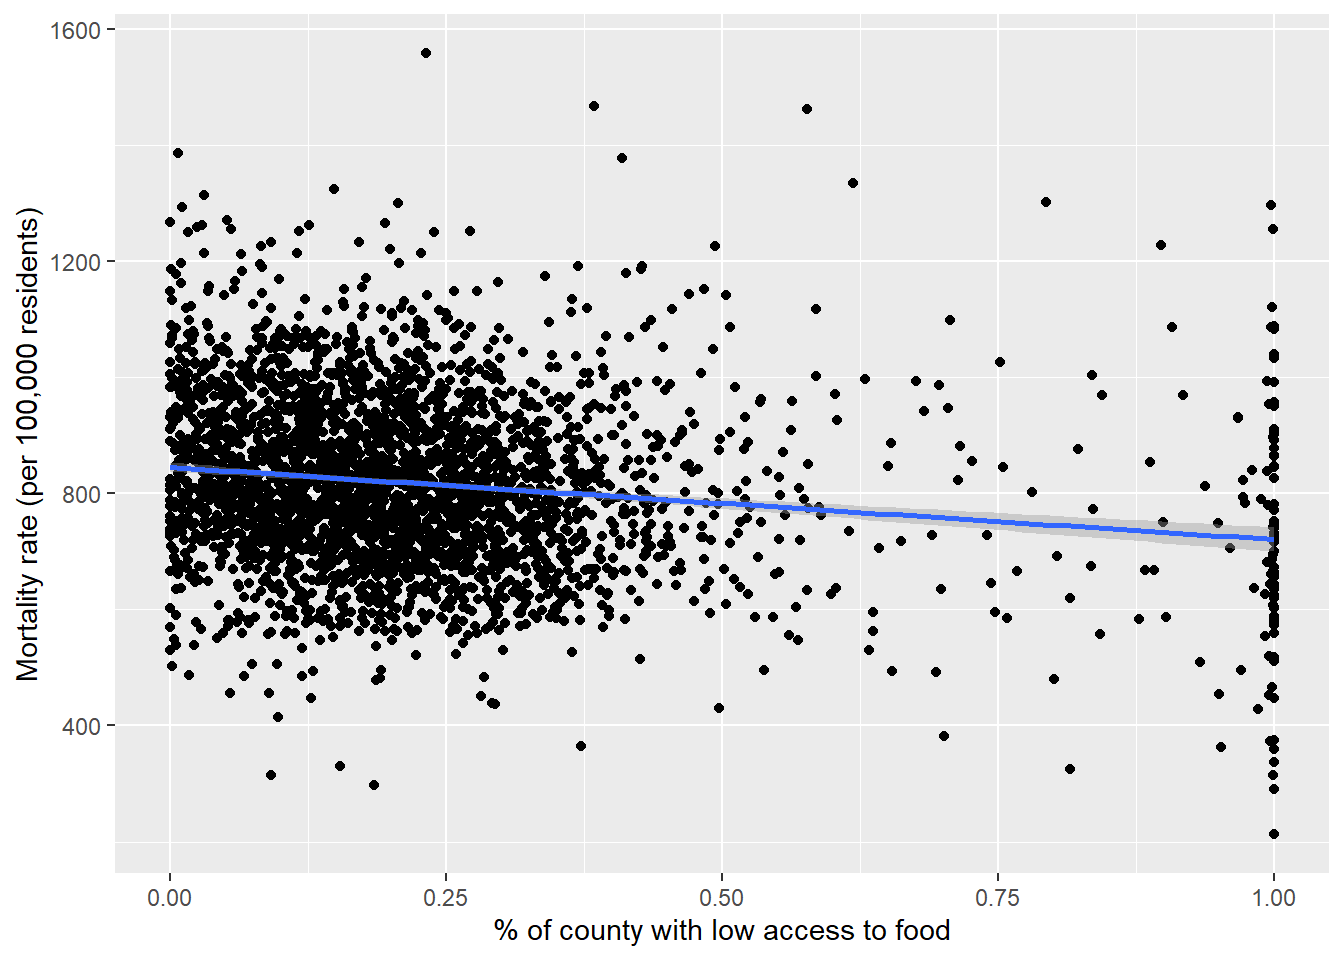
\includegraphics{Jamie-Esmond_Problem-Set-2_files/figure-latex/plot-mortality-food-1} \end{center}

\hypertarget{how-related-are-mortality-rate-and-the-prevalence-of-fast-food-restaurants}{%
\subsubsection{How related are mortality rate and the prevalence of fast
food
restaurants?}\label{how-related-are-mortality-rate-and-the-prevalence-of-fast-food-restaurants}}

\begin{Shaded}
\begin{Highlighting}[]
\NormalTok{model\_fastfood }\OtherTok{\textless{}{-}} \FunctionTok{lm}\NormalTok{(mortality\_rate }\SpecialCharTok{\textasciitilde{}}\NormalTok{ fastfood\_per\_1000,}
                         \AttributeTok{data =}\NormalTok{ food\_health)}

\FunctionTok{tidy}\NormalTok{(model\_fastfood, }\AttributeTok{conf.int =} \ConstantTok{TRUE}\NormalTok{)}
\end{Highlighting}
\end{Shaded}

\begin{verbatim}
## # A tibble: 2 x 7
##   term              estimate std.error statistic p.value conf.low conf.high
##   <chr>                <dbl>     <dbl>     <dbl>   <dbl>    <dbl>     <dbl>
## 1 (Intercept)          829.       5.67    146.    0         818.     840.  
## 2 fastfood_per_1000    -21.3      8.68     -2.45  0.0142    -38.3     -4.28
\end{verbatim}

\textbf{The mortality rate and the prevalence of fast food restaurants
are related according to this data. For every increase in fast food
restaurants per 1000 residents by one, the mortality rate drops by 21.29
per 100,000 residents. The p value is less than .05, meaning the
relationship is statistically significant. This is surprising because
one would expect an increase in the prevalence of fast food restaurants
would increase the mortality rate in the area. However, according to
this plot, most places have less than 2 fast food restaurants per 1000
residents; there are only a few areas with more than 2, and even less
with more than 4. These outliers may be skewing the results. }

\begin{Shaded}
\begin{Highlighting}[]
\FunctionTok{ggplot}\NormalTok{(food\_health, }\FunctionTok{aes}\NormalTok{(}\AttributeTok{x =}\NormalTok{ fastfood\_per\_1000, }\AttributeTok{y =}\NormalTok{ mortality\_rate)) }\SpecialCharTok{+}
  \FunctionTok{geom\_point}\NormalTok{() }\SpecialCharTok{+}
  \FunctionTok{geom\_smooth}\NormalTok{(}\AttributeTok{method =} \StringTok{"lm"}\NormalTok{) }\SpecialCharTok{+}
  \FunctionTok{labs}\NormalTok{(}\AttributeTok{x =} \StringTok{"Fast food per 1000 residents"}\NormalTok{, }
       \AttributeTok{y =} \StringTok{"Mortality rate (per 100,000 residents)"}\NormalTok{)}
\end{Highlighting}
\end{Shaded}

\begin{verbatim}
## `geom_smooth()` using formula = 'y ~ x'
\end{verbatim}

\begin{center}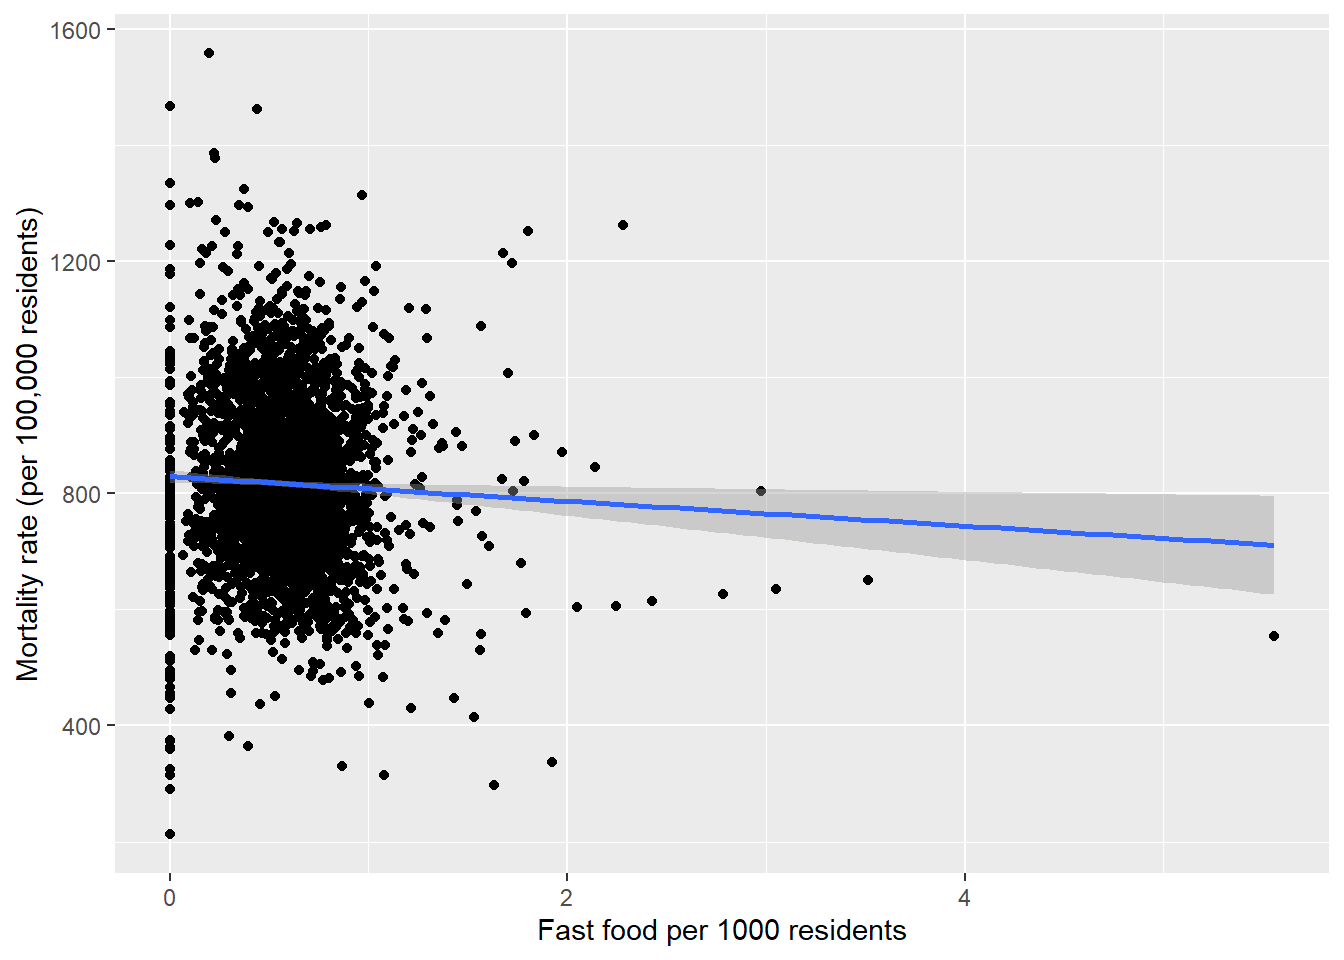
\includegraphics{Jamie-Esmond_Problem-Set-2_files/figure-latex/plot-mortality-fastfood-1} \end{center}

\hypertarget{how-related-are-mortality-rate-and-the-prevalence-of-snap-stores-per-1000-residents}{%
\subsubsection{How related are mortality rate and the prevalence of SNAP
stores per 1,000
residents?}\label{how-related-are-mortality-rate-and-the-prevalence-of-snap-stores-per-1000-residents}}

\begin{Shaded}
\begin{Highlighting}[]
\NormalTok{model\_snap }\OtherTok{\textless{}{-}} \FunctionTok{lm}\NormalTok{(mortality\_rate }\SpecialCharTok{\textasciitilde{}}\NormalTok{ snap\_stores\_per\_1000,}
                         \AttributeTok{data =}\NormalTok{ food\_health)}

\FunctionTok{tidy}\NormalTok{(model\_snap, }\AttributeTok{conf.int =} \ConstantTok{TRUE}\NormalTok{)}
\end{Highlighting}
\end{Shaded}

\begin{verbatim}
## # A tibble: 2 x 7
##   term                 estimate std.error statistic   p.value conf.low conf.high
##   <chr>                   <dbl>     <dbl>     <dbl>     <dbl>    <dbl>     <dbl>
## 1 (Intercept)              654.      6.35     103.  0             642.      667.
## 2 snap_stores_per_1000     174.      6.30      27.7 3.22e-151     162.      187.
\end{verbatim}

\textbf{The mortality rate and the prevalence of SNAP stores are related
according to this data. For every increase in SNAP stores per 1000
residents by one, the mortality rate increases by 174.49 per 100,000
residents. The p value is virtually zero, meaning the relationship is
very statistically significant. This unsurprising because one would
expect an increase in the prevalence of SNAP stores would increase the
mortality rate in the area by providing access to food to more
residents. }

\begin{Shaded}
\begin{Highlighting}[]
\FunctionTok{ggplot}\NormalTok{(food\_health, }\FunctionTok{aes}\NormalTok{(}\AttributeTok{x =}\NormalTok{ snap\_stores\_per\_1000, }\AttributeTok{y =}\NormalTok{ mortality\_rate)) }\SpecialCharTok{+}
  \FunctionTok{geom\_point}\NormalTok{() }\SpecialCharTok{+}
  \FunctionTok{geom\_smooth}\NormalTok{(}\AttributeTok{method =} \StringTok{"lm"}\NormalTok{) }\SpecialCharTok{+}
  \FunctionTok{labs}\NormalTok{(}\AttributeTok{x =} \StringTok{"SNAP stores per 1000 residents"}\NormalTok{, }
       \AttributeTok{y =} \StringTok{"Mortality rate (per 100,000 residents)"}\NormalTok{)}
\end{Highlighting}
\end{Shaded}

\begin{verbatim}
## `geom_smooth()` using formula = 'y ~ x'
\end{verbatim}

\begin{center}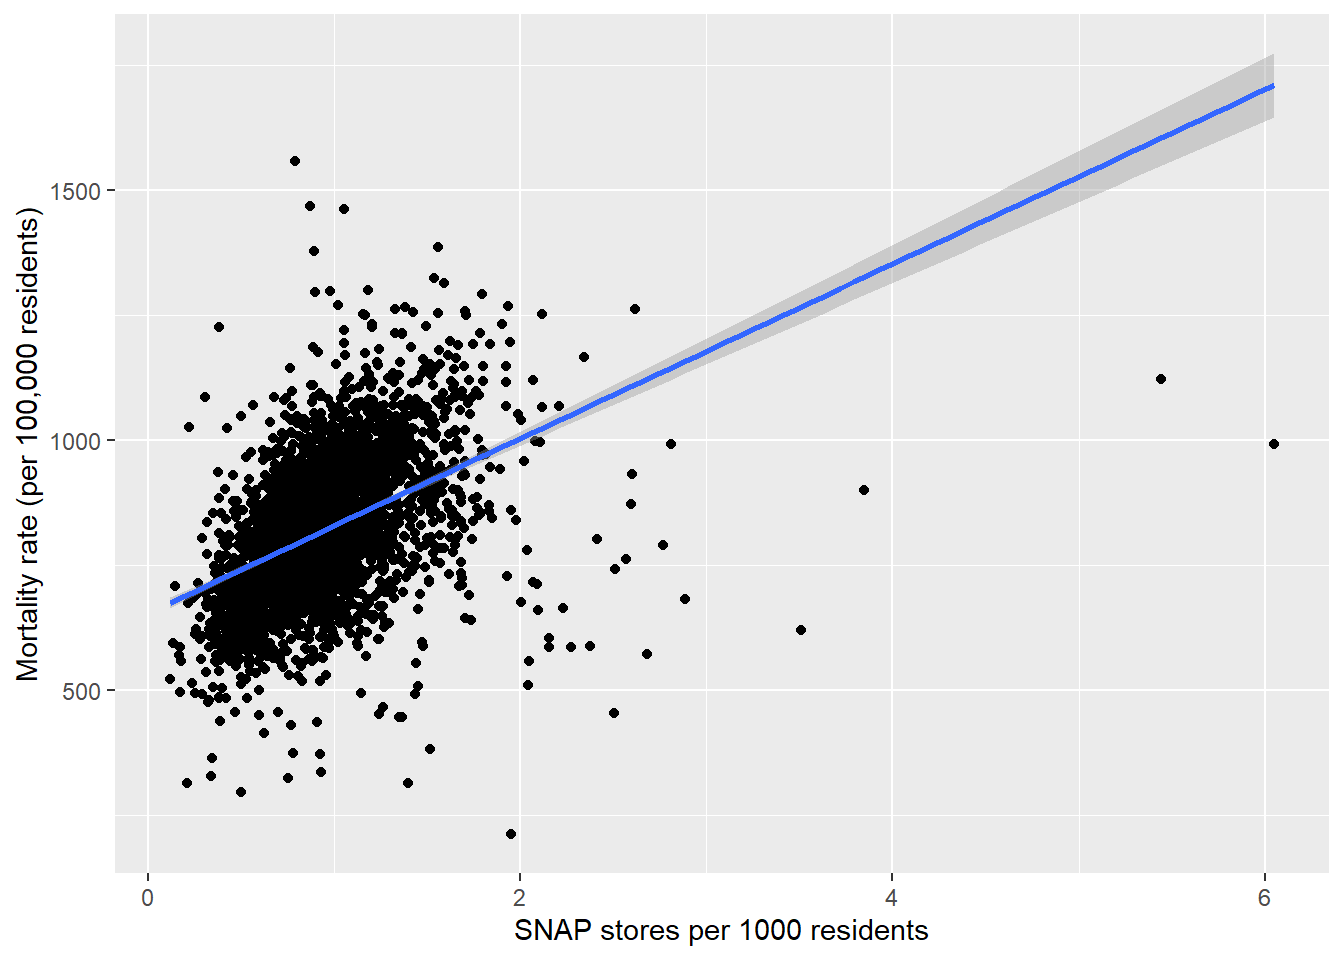
\includegraphics{Jamie-Esmond_Problem-Set-2_files/figure-latex/plot-mortality-snap-1} \end{center}

\hypertarget{how-related-are-mortality-rate-and-the-percent-of-the-county-that-voted-for-democrats-in-2016}{%
\subsubsection{How related are mortality rate and the percent of the
county that voted for Democrats in
2016?}\label{how-related-are-mortality-rate-and-the-percent-of-the-county-that-voted-for-democrats-in-2016}}

\begin{Shaded}
\begin{Highlighting}[]
\NormalTok{model\_vote }\OtherTok{\textless{}{-}} \FunctionTok{lm}\NormalTok{(mortality\_rate }\SpecialCharTok{\textasciitilde{}}\NormalTok{ per\_dem\_2016,}
                         \AttributeTok{data =}\NormalTok{ food\_health)}

\FunctionTok{tidy}\NormalTok{(model\_vote, }\AttributeTok{conf.int =} \ConstantTok{TRUE}\NormalTok{)}
\end{Highlighting}
\end{Shaded}

\begin{verbatim}
## # A tibble: 2 x 7
##   term         estimate std.error statistic  p.value conf.low conf.high
##   <chr>           <dbl>     <dbl>     <dbl>    <dbl>    <dbl>     <dbl>
## 1 (Intercept)      861.      6.05    142.   0            849.      873.
## 2 per_dem_2016    -139.     17.2      -8.13 6.36e-16    -173.     -106.
\end{verbatim}

\textbf{The mortality rate and the percent of the county that voted for
Democrats in 2016 are related according to this data. For every one
point increase in the percent of the county that voted for Democrats in
2016 per 1000 residents, the mortality rate decreased by 139.35 per
100,000 residents. The p value is virtually zero, meaning the
relationship is very statistically significant. }

\begin{Shaded}
\begin{Highlighting}[]
\FunctionTok{ggplot}\NormalTok{(food\_health, }\FunctionTok{aes}\NormalTok{(}\AttributeTok{x =}\NormalTok{ per\_dem\_2016}\SpecialCharTok{*}\DecValTok{100}\NormalTok{, }\AttributeTok{y =}\NormalTok{ mortality\_rate)) }\SpecialCharTok{+}
  \FunctionTok{geom\_point}\NormalTok{() }\SpecialCharTok{+}
  \FunctionTok{geom\_smooth}\NormalTok{(}\AttributeTok{method =} \StringTok{"lm"}\NormalTok{) }\SpecialCharTok{+}
  \FunctionTok{labs}\NormalTok{(}\AttributeTok{x =} \StringTok{"Percent of Vote for Democrats"}\NormalTok{, }
       \AttributeTok{y =} \StringTok{"Mortality rate (per 100,000 residents)"}\NormalTok{)}
\end{Highlighting}
\end{Shaded}

\begin{verbatim}
## `geom_smooth()` using formula = 'y ~ x'
\end{verbatim}

\begin{center}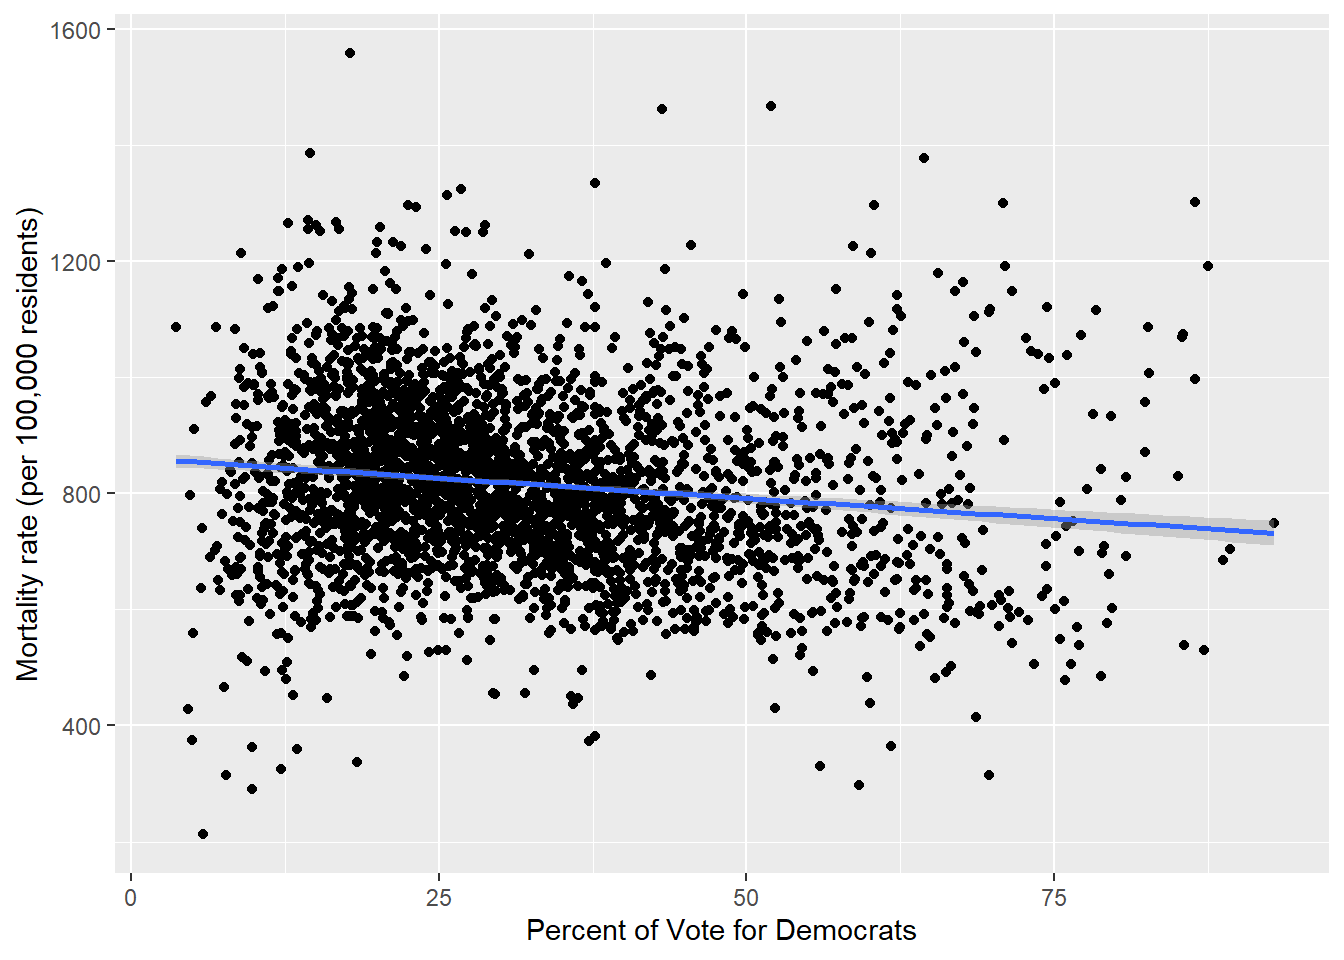
\includegraphics{Jamie-Esmond_Problem-Set-2_files/figure-latex/plot-mortality-2016-1} \end{center}

\hypertarget{models-1}{%
\subsection{Models}\label{models-1}}

\hypertarget{does-access-to-food-predict-mortality}{%
\subsubsection{Does access to food predict
mortality?}\label{does-access-to-food-predict-mortality}}

\textbf{According to this model, there is a negative relationship
between food access and mortality. When low access to food increases,
the mortality rate decreases.}

\begin{Shaded}
\begin{Highlighting}[]
\NormalTok{model\_mortality\_food }\OtherTok{\textless{}{-}} \FunctionTok{lm}\NormalTok{(mortality\_rate }\SpecialCharTok{\textasciitilde{}}\NormalTok{ pct\_low\_access\_pop,}
                           \AttributeTok{data =}\NormalTok{ food\_health)}

\FunctionTok{tidy}\NormalTok{(model\_mortality\_food, }\AttributeTok{conf.int =} \ConstantTok{TRUE}\NormalTok{)}
\end{Highlighting}
\end{Shaded}

\begin{verbatim}
## # A tibble: 2 x 7
##   term               estimate std.error statistic  p.value conf.low conf.high
##   <chr>                 <dbl>     <dbl>     <dbl>    <dbl>    <dbl>     <dbl>
## 1 (Intercept)            845.      4.06    208.   0            837.     853. 
## 2 pct_low_access_pop    -125.     13.5      -9.23 4.94e-20    -151.     -98.1
\end{verbatim}

\begin{Shaded}
\begin{Highlighting}[]
\FunctionTok{glance}\NormalTok{(model\_mortality\_food)}
\end{Highlighting}
\end{Shaded}

\begin{verbatim}
## # A tibble: 1 x 12
##   r.squared adj.r.s~1 sigma stati~2  p.value    df  logLik    AIC    BIC devia~3
##       <dbl>     <dbl> <dbl>   <dbl>    <dbl> <dbl>   <dbl>  <dbl>  <dbl>   <dbl>
## 1    0.0266    0.0263  146.    85.2 4.94e-20     1 -19948. 39901. 39920.  6.63e7
## # ... with 2 more variables: df.residual <int>, nobs <int>, and abbreviated
## #   variable names 1: adj.r.squared, 2: statistic, 3: deviance
\end{verbatim}

What happens as the percent of low access to food goes up by 1\%? Is
that significant? Again, this is backwards from what you'd expect---as
the percent of low access goes up, mortality drops. Why might that be?
How much do you trust this finding? (Hint: look at the \(R^2\) value)

\textbf{As the percent of residents with low food access increases by
one point, the mortality rate decreases by 845.31 (per 100,000
residents). This relationship is statistically significant because the p
value is virtually zero. There could be other factors that are not
displayed in this data that could be impacting mortality rates. For
example, rural counties may have less access to food because the
population is lower and residents are more likely to live further away
from grocery stores. It is unclear what the metric for ``low access to
food'' is here. According to the \(R^2\) value, low food access only
accounts for 26.6\% of the variation in mortality rate.}

\hypertarget{do-more-snap-stores-per-person-predict-mortality}{%
\subsubsection{Do more SNAP stores per person predict
mortality?}\label{do-more-snap-stores-per-person-predict-mortality}}

\begin{Shaded}
\begin{Highlighting}[]
\NormalTok{model\_mortality\_snap }\OtherTok{\textless{}{-}} \FunctionTok{lm}\NormalTok{(mortality\_rate }\SpecialCharTok{\textasciitilde{}}\NormalTok{ snap\_stores\_per\_1000,}
                           \AttributeTok{data =}\NormalTok{ food\_health)}

\FunctionTok{tidy}\NormalTok{(model\_mortality\_snap, }\AttributeTok{conf.int =} \ConstantTok{TRUE}\NormalTok{)}
\end{Highlighting}
\end{Shaded}

\begin{verbatim}
## # A tibble: 2 x 7
##   term                 estimate std.error statistic   p.value conf.low conf.high
##   <chr>                   <dbl>     <dbl>     <dbl>     <dbl>    <dbl>     <dbl>
## 1 (Intercept)              654.      6.35     103.  0             642.      667.
## 2 snap_stores_per_1000     174.      6.30      27.7 3.22e-151     162.      187.
\end{verbatim}

\begin{Shaded}
\begin{Highlighting}[]
\FunctionTok{glance}\NormalTok{(model\_mortality\_snap)}
\end{Highlighting}
\end{Shaded}

\begin{verbatim}
## # A tibble: 1 x 12
##   r.squared adj.r.~1 sigma stati~2   p.value    df  logLik    AIC    BIC devia~3
##       <dbl>    <dbl> <dbl>   <dbl>     <dbl> <dbl>   <dbl>  <dbl>  <dbl>   <dbl>
## 1     0.198    0.198  131.    768. 3.22e-151     1 -19595. 39196. 39214.  5.37e7
## # ... with 2 more variables: df.residual <int>, nobs <int>, and abbreviated
## #   variable names 1: adj.r.squared, 2: statistic, 3: deviance
\end{verbatim}

What happens as the proportion of SNAP stores goes up? Do you trust this
number more or less than low access to food?

\textbf{As the number of SNAP stores per 1000 residents increases by
one, the mortality rate increases by 174.49 (per 100,000 residents).
This relationship is statistically significant because the p value is
virtually zero. According to the \(R^2\) value, low food access only
accounts for 19.8\% of the variation in mortality rate, which is even
less than what low food access accounted for. Again, there are likely
other factors such as neighborhood characteristics and income that might
better explain this surprising result. For example, stores that accept
SNAP are more likely to be located in low income neighborhoods; people
in low income neighborhoods are more likely to be low income, and less
income decreases access to medical care, which, of course, can increase
mortality.}

\hypertarget{do-election-results-and-access-to-food-and-snap-stores-predict-mortality}{%
\subsubsection{Do election results and access to food and SNAP stores
predict
mortality?}\label{do-election-results-and-access-to-food-and-snap-stores-predict-mortality}}

RUN A MODEL THAT PREDICTS MORTALITY WITH A BUNCH OF COVARIATES
(i.e.~mortality\_rate \textasciitilde{} pct\_low\_access\_pop +
snap\_stores\_per\_1000 + per\_dem\_2016 + anything else you want to
throw in)

\begin{Shaded}
\begin{Highlighting}[]
\NormalTok{model\_mortality\_many }\OtherTok{\textless{}{-}} \FunctionTok{lm}\NormalTok{(mortality\_rate }\SpecialCharTok{\textasciitilde{}}\NormalTok{ pct\_low\_access\_pop }\SpecialCharTok{+}
\NormalTok{                                            snap\_stores\_per\_1000 }\SpecialCharTok{+}
\NormalTok{                                            fastfood\_per\_1000 }\SpecialCharTok{+}
\NormalTok{                                            per\_dem\_2016,}
                           \AttributeTok{data =}\NormalTok{ food\_health)}

\FunctionTok{tidy}\NormalTok{(model\_mortality\_many, }\AttributeTok{conf.int =} \ConstantTok{TRUE}\NormalTok{)}
\end{Highlighting}
\end{Shaded}

\begin{verbatim}
## # A tibble: 5 x 7
##   term                 estimate std.error statistic   p.value conf.low conf.high
##   <chr>                   <dbl>     <dbl>     <dbl>     <dbl>    <dbl>     <dbl>
## 1 (Intercept)             744.       8.92     83.4  0            726.     761.  
## 2 pct_low_access_pop     -170.      12.3     -13.9  1.41e- 42   -194.    -146.  
## 3 snap_stores_per_1000    181.       6.06     29.9  5.60e-173    169.     193.  
## 4 fastfood_per_1000       -17.6      7.68     -2.29 2.19e-  2    -32.7     -2.55
## 5 per_dem_2016           -149.      15.2      -9.82 1.92e- 22   -179.    -119.
\end{verbatim}

\begin{Shaded}
\begin{Highlighting}[]
\FunctionTok{glance}\NormalTok{(model\_mortality\_many)}
\end{Highlighting}
\end{Shaded}

\begin{verbatim}
## # A tibble: 1 x 12
##   r.squared adj.r.~1 sigma stati~2   p.value    df  logLik    AIC    BIC devia~3
##       <dbl>    <dbl> <dbl>   <dbl>     <dbl> <dbl>   <dbl>  <dbl>  <dbl>   <dbl>
## 1     0.266    0.265  125.    279. 3.38e-205     4 -19331. 38674. 38710.  4.86e7
## # ... with 2 more variables: df.residual <int>, nobs <int>, and abbreviated
## #   variable names 1: adj.r.squared, 2: statistic, 3: deviance
\end{verbatim}

Interpret the different coefficients. How predictive is this model
(i.e.~what's the R2)? Do you believe this model?

\textbf{When controlling for low access to food, the number of SNAP
stores per 1000 residents, and the prevalence of fast food restaurants,
as the percent of the county who voted Democrat in 2016 increases by one
point, the mortality rate decreases by 149.2 (per 100,000 residents). As
the percent of residents with low access to food increases, the
mortality rate decreases when holding all other variables constant. The
prevalence of SNAP stores has a positive relationship with the mortality
rate, but the prevalence of fast food restaurants' relationship is
negative when the other variables are held constant. These relationships
are statistically significant because the p values are all virtually
zero. In summary, low access to food and more fast food decrease the
mortality rate, and the presence of SNAP stores increases the mortality
rate. According to the adjusted \(R^2\) value, these factors only
account for 26.5\% of the variation in mortality rate. What accounts for
the other 73.5\% of the mortality rate? This model does not include
enough other influential variables that are necessary to access the
factors that lead to a high mortality rate.}

\hypertarget{mortality-contolling-for-state-differences}{%
\subsubsection{Mortality, contolling for state
differences}\label{mortality-contolling-for-state-differences}}

RUN A MODEL with some number of plausible independent/explanatory
variables. Include \texttt{state} as one of them

\begin{Shaded}
\begin{Highlighting}[]
\CommentTok{\# Add other explanatory variables here}
\NormalTok{model\_with\_state }\OtherTok{\textless{}{-}} \FunctionTok{lm}\NormalTok{(mortality\_rate }\SpecialCharTok{\textasciitilde{}}\NormalTok{ pct\_low\_access\_pop }\SpecialCharTok{+}\NormalTok{ state,}
                       \AttributeTok{data =}\NormalTok{ food\_health)}

\CommentTok{\# This table is 50+ rows long! While it might be interesting to see changes in}
\CommentTok{\# intercept in relation to Alaska (the omitted state here), like how Alabama\textquotesingle{}s}
\CommentTok{\# mortality rate is 137 higher than Alaska\textquotesingle{}s while DC\textquotesingle{}s is 84 lower, it\textquotesingle{}s not}
\CommentTok{\# super helpful. Controlling for state does capture some of the state{-}specific}
\CommentTok{\# reasons for varying mortality though, so it\textquotesingle{}s good to include. We just don\textquotesingle{}t}
\CommentTok{\# really need to see all those coefficients. To remove them from this table of}
\CommentTok{\# results, filter them out. The "!" in R means "not", so here we\textquotesingle{}re only looking}
\CommentTok{\# at rows that don\textquotesingle{}t start with "state"}
\FunctionTok{tidy}\NormalTok{(model\_with\_state, }\AttributeTok{conf.int =} \ConstantTok{TRUE}\NormalTok{) }\SpecialCharTok{\%\textgreater{}\%} 
  \FunctionTok{filter}\NormalTok{(}\SpecialCharTok{!}\FunctionTok{str\_starts}\NormalTok{(term, }\StringTok{"state"}\NormalTok{))}
\end{Highlighting}
\end{Shaded}

\begin{verbatim}
## # A tibble: 2 x 7
##   term               estimate std.error statistic   p.value conf.low conf.high
##   <chr>                 <dbl>     <dbl>     <dbl>     <dbl>    <dbl>     <dbl>
## 1 (Intercept)           835.       23.3     35.9  8.30e-236    790.      881. 
## 2 pct_low_access_pop    -54.7      12.1     -4.50 6.95e-  6    -78.5     -30.9
\end{verbatim}

\begin{Shaded}
\begin{Highlighting}[]
\NormalTok{model\_mortality\_many\_state }\OtherTok{\textless{}{-}} \FunctionTok{lm}\NormalTok{(mortality\_rate }\SpecialCharTok{\textasciitilde{}}\NormalTok{ pct\_low\_access\_pop }\SpecialCharTok{+}
\NormalTok{                                            snap\_stores\_per\_1000 }\SpecialCharTok{+}
\NormalTok{                                            fastfood\_per\_1000 }\SpecialCharTok{+}
\NormalTok{                                            per\_dem\_2016 }\SpecialCharTok{+}
\NormalTok{                                            state,}
                           \AttributeTok{data =}\NormalTok{ food\_health)}

\FunctionTok{tidy}\NormalTok{(model\_mortality\_many\_state, }\AttributeTok{conf.int =} \ConstantTok{TRUE}\NormalTok{) }\SpecialCharTok{\%\textgreater{}\%} 
  \FunctionTok{filter}\NormalTok{(}\SpecialCharTok{!}\FunctionTok{str\_starts}\NormalTok{(term, }\StringTok{"state"}\NormalTok{))}
\end{Highlighting}
\end{Shaded}

\begin{verbatim}
## # A tibble: 5 x 7
##   term                 estimate std.error statistic   p.value conf.low conf.high
##   <chr>                   <dbl>     <dbl>     <dbl>     <dbl>    <dbl>     <dbl>
## 1 (Intercept)             652.      24.0      27.2  8.32e-146    605.     699.  
## 2 pct_low_access_pop      -97.2     11.6      -8.39 7.08e- 17   -120.     -74.5 
## 3 snap_stores_per_1000    135.       5.68     23.7  5.34e-114    123.     146.  
## 4 fastfood_per_1000       -17.0      6.72     -2.52 1.17e-  2    -30.1     -3.78
## 5 per_dem_2016            -63.9     15.5      -4.13 3.65e-  5    -94.2    -33.6
\end{verbatim}

\textbf{When controlling for low access to food, the number of SNAP
stores per 1000 residents, the prevalence of fast food restaurants, and
state, as the percent of the county who voted Democrat in 2016 increases
by one point, the mortality rate decreases by 63.88 (per 100,000
residents), which is less of a decrease than without controlling for
state. As the percent of residents with low access to food increases,
the mortality rate still decreases when holding all other variables
constant, but by much less. The prevalence of SNAP stores still has a
positive relationship with the mortality rate, and the prevalence of
fast food restaurants' relationship is still negative when the other
variables are held constant, but there is less of a difference. These
relationships are still statistically significant because the p values
are all virtually zero. In summary, low access to food and more fast
food decrease the mortality rate, and the presence of SNAP stores
increases the mortality rate, but less so when you control for state.}

\hypertarget{all-models-at-the-same-time-1}{%
\subsection{All models at the same
time}\label{all-models-at-the-same-time-1}}

\begin{Shaded}
\begin{Highlighting}[]
\CommentTok{\# Right now there are only two models here. Add the others from above (whatever }
\CommentTok{\# you called them) like so: }
\CommentTok{\# modelsummary(list(model\_mortality\_food, some\_other\_model, yet\_another\_model, etc))}

\CommentTok{\# Also, by default, modelsummary will include all the state coefficients, which}
\CommentTok{\# we don\textquotesingle{}t want. We can omit specific coefficients with the \textasciigrave{}coef\_omit\textasciigrave{}}
\CommentTok{\# argument. The \^{} character means it\textquotesingle{}ll omit coefficients that *start with*}
\CommentTok{\# "state". Without \^{}, it would omit any coefficient where the characters "state"}
\CommentTok{\# appeared anywhere in the name, which might be too greedy}
\NormalTok{notes }\OtherTok{\textless{}{-}} \FunctionTok{c}\NormalTok{(}\StringTok{"t statistics in parentheses}\SpecialCharTok{\textbackslash{}n}\StringTok{"}\NormalTok{,}
           \StringTok{"+ p \textless{} 0.1, * p \textless{} 0.05, ** p \textless{} 0.01, *** p \textless{} 0.001"}\NormalTok{)}

\FunctionTok{modelsummary}\NormalTok{(}\FunctionTok{list}\NormalTok{(}\StringTok{"Model 1"}\OtherTok{=}\NormalTok{model\_snap,}
                  \StringTok{"Model 2"}\OtherTok{=}\NormalTok{model\_vote,}
                  \StringTok{"Model 3"}\OtherTok{=}\NormalTok{model\_mortality\_food,}
                  \StringTok{"Model 4"}\OtherTok{=}\NormalTok{model\_mortality\_snap,}
                  \StringTok{"Model 5"}\OtherTok{=}\NormalTok{model\_mortality\_many,}
                  \StringTok{"Model 6"}\OtherTok{=}\NormalTok{model\_with\_state,}
                  \StringTok{"Model 7"}\OtherTok{=}\NormalTok{model\_mortality\_many\_state),}
             \AttributeTok{coef\_omit =} \StringTok{"\^{}state"}\NormalTok{,}
             \AttributeTok{coef\_rename =} \FunctionTok{c}\NormalTok{(}\AttributeTok{pct\_low\_access\_pop =} \StringTok{"Percent of the county\textquotesingle{}s population with low access to food"}\NormalTok{, }
                             \AttributeTok{snap\_stores\_per\_1000 =} \StringTok{"Number of stores that accept SNAP in a county (per 1,000 residents)"}\NormalTok{, }
                             \AttributeTok{fastfood\_per\_1000 =} \StringTok{"Number of fast food stores in a county (per 1,000 residents"}\NormalTok{, }
                             \AttributeTok{per\_dem\_2016 =} \StringTok{"Percent of the county that voted for Clinton in 2016"}\NormalTok{),}
             \AttributeTok{output =} \StringTok{"kableExtra"}\NormalTok{,}
             \AttributeTok{estimate =} \StringTok{"\{estimate\} \{stars\}"}\NormalTok{,}
             \AttributeTok{statistic =} \StringTok{"statistic"}\NormalTok{,}
             \AttributeTok{title =} \StringTok{"Mortality Rates and Access to Food"}\NormalTok{,}
             \AttributeTok{fmt =}  \DecValTok{2}\NormalTok{) }\SpecialCharTok{\%\textgreater{}\%} 
    \FunctionTok{row\_spec}\NormalTok{(}\FunctionTok{c}\NormalTok{(}\DecValTok{1}\NormalTok{,}\DecValTok{3}\NormalTok{,}\DecValTok{5}\NormalTok{,}\DecValTok{7}\NormalTok{,}\DecValTok{9}\NormalTok{), }\AttributeTok{background =} \StringTok{"lightyellow"}\NormalTok{) }\SpecialCharTok{\%\textgreater{}\%} 
    \FunctionTok{footnote}\NormalTok{(}\AttributeTok{general =}\NormalTok{ notes, }\AttributeTok{footnote\_as\_chunk =} \ConstantTok{TRUE}\NormalTok{)}
\end{Highlighting}
\end{Shaded}

\begin{table}

\caption{\label{tab:everything-together}Mortality Rates and Access to Food}
\centering
\begin{tabular}[t]{lccccccc}
\toprule
  & Model 1 & Model 2 & Model 3 & Model 4 & Model 5 & Model 6 & Model 7\\
\midrule
\cellcolor{lightyellow}{(Intercept)} & \cellcolor{lightyellow}{\num{654.37} ***} & \cellcolor{lightyellow}{\num{861.34} ***} & \cellcolor{lightyellow}{\num{845.31} ***} & \cellcolor{lightyellow}{\num{654.37} ***} & \cellcolor{lightyellow}{\num{743.85} ***} & \cellcolor{lightyellow}{\num{835.29} ***} & \cellcolor{lightyellow}{\num{651.97} ***}\\
 & (\num{103.05}) & (\num{142.43}) & (\num{208.42}) & (\num{103.05}) & (\num{83.41}) & (\num{35.89}) & (\num{27.18})\\
\cellcolor{lightyellow}{Number of stores that accept SNAP in a county (per 1,000 residents)} & \cellcolor{lightyellow}{\num{174.49} ***} & \cellcolor{lightyellow}{} & \cellcolor{lightyellow}{} & \cellcolor{lightyellow}{\num{174.49} ***} & \cellcolor{lightyellow}{\num{181.28} ***} & \cellcolor{lightyellow}{} & \cellcolor{lightyellow}{\num{134.63} ***}\\
 & (\num{27.71}) &  &  & (\num{27.71}) & (\num{29.92}) &  & (\num{23.69})\\
\cellcolor{lightyellow}{Percent of the county that voted for Clinton in 2016} & \cellcolor{lightyellow}{} & \cellcolor{lightyellow}{\num{-139.35} ***} & \cellcolor{lightyellow}{} & \cellcolor{lightyellow}{} & \cellcolor{lightyellow}{\num{-149.20} ***} & \cellcolor{lightyellow}{} & \cellcolor{lightyellow}{\num{-63.88} ***}\\
 &  & (\num{-8.13}) &  &  & (\num{-9.82}) &  & (\num{-4.13})\\
\cellcolor{lightyellow}{Percent of the county's population with low access to food} & \cellcolor{lightyellow}{} & \cellcolor{lightyellow}{} & \cellcolor{lightyellow}{\num{-124.52} ***} & \cellcolor{lightyellow}{} & \cellcolor{lightyellow}{\num{-170.35} ***} & \cellcolor{lightyellow}{\num{-54.66} ***} & \cellcolor{lightyellow}{\num{-97.19} ***}\\
 &  &  & (\num{-9.23}) &  & (\num{-13.89}) & (\num{-4.50}) & (\num{-8.39})\\
\cellcolor{lightyellow}{Number of fast food stores in a county (per 1,000 residents} & \cellcolor{lightyellow}{} & \cellcolor{lightyellow}{} & \cellcolor{lightyellow}{} & \cellcolor{lightyellow}{} & \cellcolor{lightyellow}{\num{-17.62} *} & \cellcolor{lightyellow}{} & \cellcolor{lightyellow}{\num{-16.96} *}\\
 &  &  &  &  & (\num{-2.29}) &  & (\num{-2.52})\\
\midrule
Num.Obs. & \num{3112} & \num{3135} & \num{3116} & \num{3112} & \num{3093} & \num{3116} & \num{3093}\\
R2 & \num{0.198} & \num{0.021} & \num{0.027} & \num{0.198} & \num{0.266} & \num{0.384} & \num{0.488}\\
R2 Adj. & \num{0.198} & \num{0.020} & \num{0.026} & \num{0.198} & \num{0.265} & \num{0.374} & \num{0.479}\\
AIC & \num{39196.3} & \num{40180.0} & \num{39901.5} & \num{39196.3} & \num{38673.5} & \num{38576.6} & \num{37658.7}\\
BIC & \num{39214.4} & \num{40198.1} & \num{39919.6} & \num{39214.4} & \num{38709.8} & \num{38897.0} & \num{37996.8}\\
Log.Lik. & \num{-19595.130} & \num{-20086.999} & \num{-19947.736} & \num{-19595.130} & \num{-19330.772} & \num{-19235.313} & \num{-18773.354}\\
RMSE & \num{131.33} & \num{146.70} & \num{145.88} & \num{131.33} & \num{125.32} & \num{116.06} & \num{104.66}\\
\bottomrule
\multicolumn{8}{l}{\rule{0pt}{1em}\textit{Note: } makecell[l]{t statistics in parentheses\} + p < 0.1, * p < 0.05, ** p < 0.01, *** p < 0.001}\\
\end{tabular}
\end{table}

\end{document}
